\documentclass[a4paper]{article}

% if you need to pass options to natbib, use, e.g.:
%     \PassOptionsToPackage{numbers, compress}{natbib}
% before loading neurips_2022


% ready for submission
%\usepackage{ofu_xai_2022}

% SOURCE: https://github.com/goodfeli/dlbook_notation/blob/master/math_commands.tex
% Quote from github "We make them freely available for anyone to use."

\usepackage{amsmath,amsfonts,bm}


%%%%% NEW MATH DEFINITIONS %%%%%

% Mark sections of captions for referring to divisions of figures
\newcommand{\figleft}{{\em (Left)}}
\newcommand{\figcenter}{{\em (Center)}}
\newcommand{\figright}{{\em (Right)}}
\newcommand{\figtop}{{\em (Top)}}
\newcommand{\figbottom}{{\em (Bottom)}}
\newcommand{\captiona}{{\em (a)}}
\newcommand{\captionb}{{\em (b)}}
\newcommand{\captionc}{{\em (c)}}
\newcommand{\captiond}{{\em (d)}}

% Highlight a newly defined term
\newcommand{\newterm}[1]{{\bf #1}}


% Figure reference, lower-case.
\def\figref#1{figure~\ref{#1}}
% Figure reference, capital. For start of sentence
\def\Figref#1{Figure~\ref{#1}}
\def\twofigref#1#2{figures \ref{#1} and \ref{#2}}
\def\quadfigref#1#2#3#4{figures \ref{#1}, \ref{#2}, \ref{#3} and \ref{#4}}
% Section reference, lower-case.
\def\secref#1{section~\ref{#1}}
% Section reference, capital.
\def\Secref#1{Section~\ref{#1}}
% Reference to two sections.
\def\twosecrefs#1#2{sections \ref{#1} and \ref{#2}}
% Reference to three sections.
\def\secrefs#1#2#3{sections \ref{#1}, \ref{#2} and \ref{#3}}
% Reference to an equation, lower-case.
\def\eqref#1{equation~\ref{#1}}
% Reference to an equation, upper case
\def\Eqref#1{Equation~\ref{#1}}
% A raw reference to an equation---avoid using if possible
\def\plaineqref#1{\ref{#1}}
% Reference to a chapter, lower-case.
\def\chapref#1{chapter~\ref{#1}}
% Reference to an equation, upper case.
\def\Chapref#1{Chapter~\ref{#1}}
% Reference to a range of chapters
\def\rangechapref#1#2{chapters\ref{#1}--\ref{#2}}
% Reference to an algorithm, lower-case.
\def\algref#1{algorithm~\ref{#1}}
% Reference to an algorithm, upper case.
\def\Algref#1{Algorithm~\ref{#1}}
\def\twoalgref#1#2{algorithms \ref{#1} and \ref{#2}}
\def\Twoalgref#1#2{Algorithms \ref{#1} and \ref{#2}}
% Reference to a part, lower case
\def\partref#1{part~\ref{#1}}
% Reference to a part, upper case
\def\Partref#1{Part~\ref{#1}}
\def\twopartref#1#2{parts \ref{#1} and \ref{#2}}

\def\ceil#1{\lceil #1 \rceil}
\def\floor#1{\lfloor #1 \rfloor}
\def\1{\bm{1}}
\newcommand{\train}{\mathcal{D}}
\newcommand{\valid}{\mathcal{D_{\mathrm{valid}}}}
\newcommand{\test}{\mathcal{D_{\mathrm{test}}}}

\def\eps{{\epsilon}}


% Random variables
\def\reta{{\textnormal{$\eta$}}}
\def\ra{{\textnormal{a}}}
\def\rb{{\textnormal{b}}}
\def\rc{{\textnormal{c}}}
\def\rd{{\textnormal{d}}}
\def\re{{\textnormal{e}}}
\def\rf{{\textnormal{f}}}
\def\rg{{\textnormal{g}}}
\def\rh{{\textnormal{h}}}
\def\ri{{\textnormal{i}}}
\def\rj{{\textnormal{j}}}
\def\rk{{\textnormal{k}}}
\def\rl{{\textnormal{l}}}
% rm is already a command, just don't name any random variables m
\def\rn{{\textnormal{n}}}
\def\ro{{\textnormal{o}}}
\def\rp{{\textnormal{p}}}
\def\rq{{\textnormal{q}}}
\def\rr{{\textnormal{r}}}
\def\rs{{\textnormal{s}}}
\def\rt{{\textnormal{t}}}
\def\ru{{\textnormal{u}}}
\def\rv{{\textnormal{v}}}
\def\rw{{\textnormal{w}}}
\def\rx{{\textnormal{x}}}
\def\ry{{\textnormal{y}}}
\def\rz{{\textnormal{z}}}

% Random vectors
\def\rvepsilon{{\mathbf{\epsilon}}}
\def\rvtheta{{\mathbf{\theta}}}
\def\rva{{\mathbf{a}}}
\def\rvb{{\mathbf{b}}}
\def\rvc{{\mathbf{c}}}
\def\rvd{{\mathbf{d}}}
\def\rve{{\mathbf{e}}}
\def\rvf{{\mathbf{f}}}
\def\rvg{{\mathbf{g}}}
\def\rvh{{\mathbf{h}}}
\def\rvu{{\mathbf{i}}}
\def\rvj{{\mathbf{j}}}
\def\rvk{{\mathbf{k}}}
\def\rvl{{\mathbf{l}}}
\def\rvm{{\mathbf{m}}}
\def\rvn{{\mathbf{n}}}
\def\rvo{{\mathbf{o}}}
\def\rvp{{\mathbf{p}}}
\def\rvq{{\mathbf{q}}}
\def\rvr{{\mathbf{r}}}
\def\rvs{{\mathbf{s}}}
\def\rvt{{\mathbf{t}}}
\def\rvu{{\mathbf{u}}}
\def\rvv{{\mathbf{v}}}
\def\rvw{{\mathbf{w}}}
\def\rvx{{\mathbf{x}}}
\def\rvy{{\mathbf{y}}}
\def\rvz{{\mathbf{z}}}

% Elements of random vectors
\def\erva{{\textnormal{a}}}
\def\ervb{{\textnormal{b}}}
\def\ervc{{\textnormal{c}}}
\def\ervd{{\textnormal{d}}}
\def\erve{{\textnormal{e}}}
\def\ervf{{\textnormal{f}}}
\def\ervg{{\textnormal{g}}}
\def\ervh{{\textnormal{h}}}
\def\ervi{{\textnormal{i}}}
\def\ervj{{\textnormal{j}}}
\def\ervk{{\textnormal{k}}}
\def\ervl{{\textnormal{l}}}
\def\ervm{{\textnormal{m}}}
\def\ervn{{\textnormal{n}}}
\def\ervo{{\textnormal{o}}}
\def\ervp{{\textnormal{p}}}
\def\ervq{{\textnormal{q}}}
\def\ervr{{\textnormal{r}}}
\def\ervs{{\textnormal{s}}}
\def\ervt{{\textnormal{t}}}
\def\ervu{{\textnormal{u}}}
\def\ervv{{\textnormal{v}}}
\def\ervw{{\textnormal{w}}}
\def\ervx{{\textnormal{x}}}
\def\ervy{{\textnormal{y}}}
\def\ervz{{\textnormal{z}}}

% Random matrices
\def\rmA{{\mathbf{A}}}
\def\rmB{{\mathbf{B}}}
\def\rmC{{\mathbf{C}}}
\def\rmD{{\mathbf{D}}}
\def\rmE{{\mathbf{E}}}
\def\rmF{{\mathbf{F}}}
\def\rmG{{\mathbf{G}}}
\def\rmH{{\mathbf{H}}}
\def\rmI{{\mathbf{I}}}
\def\rmJ{{\mathbf{J}}}
\def\rmK{{\mathbf{K}}}
\def\rmL{{\mathbf{L}}}
\def\rmM{{\mathbf{M}}}
\def\rmN{{\mathbf{N}}}
\def\rmO{{\mathbf{O}}}
\def\rmP{{\mathbf{P}}}
\def\rmQ{{\mathbf{Q}}}
\def\rmR{{\mathbf{R}}}
\def\rmS{{\mathbf{S}}}
\def\rmT{{\mathbf{T}}}
\def\rmU{{\mathbf{U}}}
\def\rmV{{\mathbf{V}}}
\def\rmW{{\mathbf{W}}}
\def\rmX{{\mathbf{X}}}
\def\rmY{{\mathbf{Y}}}
\def\rmZ{{\mathbf{Z}}}

% Elements of random matrices
\def\ermA{{\textnormal{A}}}
\def\ermB{{\textnormal{B}}}
\def\ermC{{\textnormal{C}}}
\def\ermD{{\textnormal{D}}}
\def\ermE{{\textnormal{E}}}
\def\ermF{{\textnormal{F}}}
\def\ermG{{\textnormal{G}}}
\def\ermH{{\textnormal{H}}}
\def\ermI{{\textnormal{I}}}
\def\ermJ{{\textnormal{J}}}
\def\ermK{{\textnormal{K}}}
\def\ermL{{\textnormal{L}}}
\def\ermM{{\textnormal{M}}}
\def\ermN{{\textnormal{N}}}
\def\ermO{{\textnormal{O}}}
\def\ermP{{\textnormal{P}}}
\def\ermQ{{\textnormal{Q}}}
\def\ermR{{\textnormal{R}}}
\def\ermS{{\textnormal{S}}}
\def\ermT{{\textnormal{T}}}
\def\ermU{{\textnormal{U}}}
\def\ermV{{\textnormal{V}}}
\def\ermW{{\textnormal{W}}}
\def\ermX{{\textnormal{X}}}
\def\ermY{{\textnormal{Y}}}
\def\ermZ{{\textnormal{Z}}}

% Vectors
\def\vzero{{\bm{0}}}
\def\vone{{\bm{1}}}
\def\vmu{{\bm{\mu}}}
\def\vtheta{{\bm{\theta}}}
\def\va{{\bm{a}}}
\def\vb{{\bm{b}}}
\def\vc{{\bm{c}}}
\def\vd{{\bm{d}}}
\def\ve{{\bm{e}}}
\def\vf{{\bm{f}}}
\def\vg{{\bm{g}}}
\def\vh{{\bm{h}}}
\def\vi{{\bm{i}}}
\def\vj{{\bm{j}}}
\def\vk{{\bm{k}}}
\def\vl{{\bm{l}}}
\def\vm{{\bm{m}}}
\def\vn{{\bm{n}}}
\def\vo{{\bm{o}}}
\def\vp{{\bm{p}}}
\def\vq{{\bm{q}}}
\def\vr{{\bm{r}}}
\def\vs{{\bm{s}}}
\def\vt{{\bm{t}}}
\def\vu{{\bm{u}}}
\def\vv{{\bm{v}}}
\def\vw{{\bm{w}}}
\def\vx{{\bm{x}}}
\def\vy{{\bm{y}}}
\def\vz{{\bm{z}}}

% Elements of vectors
\def\evalpha{{\alpha}}
\def\evbeta{{\beta}}
\def\evepsilon{{\epsilon}}
\def\evlambda{{\lambda}}
\def\evomega{{\omega}}
\def\evmu{{\mu}}
\def\evpsi{{\psi}}
\def\evsigma{{\sigma}}
\def\evtheta{{\theta}}
\def\eva{{a}}
\def\evb{{b}}
\def\evc{{c}}
\def\evd{{d}}
\def\eve{{e}}
\def\evf{{f}}
\def\evg{{g}}
\def\evh{{h}}
\def\evi{{i}}
\def\evj{{j}}
\def\evk{{k}}
\def\evl{{l}}
\def\evm{{m}}
\def\evn{{n}}
\def\evo{{o}}
\def\evp{{p}}
\def\evq{{q}}
\def\evr{{r}}
\def\evs{{s}}
\def\evt{{t}}
\def\evu{{u}}
\def\evv{{v}}
\def\evw{{w}}
\def\evx{{x}}
\def\evy{{y}}
\def\evz{{z}}

% Matrix
\def\mA{{\bm{A}}}
\def\mB{{\bm{B}}}
\def\mC{{\bm{C}}}
\def\mD{{\bm{D}}}
\def\mE{{\bm{E}}}
\def\mF{{\bm{F}}}
\def\mG{{\bm{G}}}
\def\mH{{\bm{H}}}
\def\mI{{\bm{I}}}
\def\mJ{{\bm{J}}}
\def\mK{{\bm{K}}}
\def\mL{{\bm{L}}}
\def\mM{{\bm{M}}}
\def\mN{{\bm{N}}}
\def\mO{{\bm{O}}}
\def\mP{{\bm{P}}}
\def\mQ{{\bm{Q}}}
\def\mR{{\bm{R}}}
\def\mS{{\bm{S}}}
\def\mT{{\bm{T}}}
\def\mU{{\bm{U}}}
\def\mV{{\bm{V}}}
\def\mW{{\bm{W}}}
\def\mX{{\bm{X}}}
\def\mY{{\bm{Y}}}
\def\mZ{{\bm{Z}}}
\def\mBeta{{\bm{\beta}}}
\def\mPhi{{\bm{\Phi}}}
\def\mLambda{{\bm{\Lambda}}}
\def\mSigma{{\bm{\Sigma}}}

% Tensor
\DeclareMathAlphabet{\mathsfit}{\encodingdefault}{\sfdefault}{m}{sl}
\SetMathAlphabet{\mathsfit}{bold}{\encodingdefault}{\sfdefault}{bx}{n}
\newcommand{\tens}[1]{\bm{\mathsfit{#1}}}
\def\tA{{\tens{A}}}
\def\tB{{\tens{B}}}
\def\tC{{\tens{C}}}
\def\tD{{\tens{D}}}
\def\tE{{\tens{E}}}
\def\tF{{\tens{F}}}
\def\tG{{\tens{G}}}
\def\tH{{\tens{H}}}
\def\tI{{\tens{I}}}
\def\tJ{{\tens{J}}}
\def\tK{{\tens{K}}}
\def\tL{{\tens{L}}}
\def\tM{{\tens{M}}}
\def\tN{{\tens{N}}}
\def\tO{{\tens{O}}}
\def\tP{{\tens{P}}}
\def\tQ{{\tens{Q}}}
\def\tR{{\tens{R}}}
\def\tS{{\tens{S}}}
\def\tT{{\tens{T}}}
\def\tU{{\tens{U}}}
\def\tV{{\tens{V}}}
\def\tW{{\tens{W}}}
\def\tX{{\tens{X}}}
\def\tY{{\tens{Y}}}
\def\tZ{{\tens{Z}}}


% Graph
\def\gA{{\mathcal{A}}}
\def\gB{{\mathcal{B}}}
\def\gC{{\mathcal{C}}}
\def\gD{{\mathcal{D}}}
\def\gE{{\mathcal{E}}}
\def\gF{{\mathcal{F}}}
\def\gG{{\mathcal{G}}}
\def\gH{{\mathcal{H}}}
\def\gI{{\mathcal{I}}}
\def\gJ{{\mathcal{J}}}
\def\gK{{\mathcal{K}}}
\def\gL{{\mathcal{L}}}
\def\gM{{\mathcal{M}}}
\def\gN{{\mathcal{N}}}
\def\gO{{\mathcal{O}}}
\def\gP{{\mathcal{P}}}
\def\gQ{{\mathcal{Q}}}
\def\gR{{\mathcal{R}}}
\def\gS{{\mathcal{S}}}
\def\gT{{\mathcal{T}}}
\def\gU{{\mathcal{U}}}
\def\gV{{\mathcal{V}}}
\def\gW{{\mathcal{W}}}
\def\gX{{\mathcal{X}}}
\def\gY{{\mathcal{Y}}}
\def\gZ{{\mathcal{Z}}}

% Sets
\def\sA{{\mathbb{A}}}
\def\sB{{\mathbb{B}}}
\def\sC{{\mathbb{C}}}
\def\sD{{\mathbb{D}}}
% Don't use a set called E, because this would be the same as our symbol
% for expectation.
\def\sF{{\mathbb{F}}}
\def\sG{{\mathbb{G}}}
\def\sH{{\mathbb{H}}}
\def\sI{{\mathbb{I}}}
\def\sJ{{\mathbb{J}}}
\def\sK{{\mathbb{K}}}
\def\sL{{\mathbb{L}}}
\def\sM{{\mathbb{M}}}
\def\sN{{\mathbb{N}}}
\def\sO{{\mathbb{O}}}
\def\sP{{\mathbb{P}}}
\def\sQ{{\mathbb{Q}}}
\def\sR{{\mathbb{R}}}
\def\sS{{\mathbb{S}}}
\def\sT{{\mathbb{T}}}
\def\sU{{\mathbb{U}}}
\def\sV{{\mathbb{V}}}
\def\sW{{\mathbb{W}}}
\def\sX{{\mathbb{X}}}
\def\sY{{\mathbb{Y}}}
\def\sZ{{\mathbb{Z}}}

% Entries of a matrix
\def\emLambda{{\Lambda}}
\def\emA{{A}}
\def\emB{{B}}
\def\emC{{C}}
\def\emD{{D}}
\def\emE{{E}}
\def\emF{{F}}
\def\emG{{G}}
\def\emH{{H}}
\def\emI{{I}}
\def\emJ{{J}}
\def\emK{{K}}
\def\emL{{L}}
\def\emM{{M}}
\def\emN{{N}}
\def\emO{{O}}
\def\emP{{P}}
\def\emQ{{Q}}
\def\emR{{R}}
\def\emS{{S}}
\def\emT{{T}}
\def\emU{{U}}
\def\emV{{V}}
\def\emW{{W}}
\def\emX{{X}}
\def\emY{{Y}}
\def\emZ{{Z}}
\def\emSigma{{\Sigma}}

% entries of a tensor
% Same font as tensor, without \bm wrapper
\newcommand{\etens}[1]{\mathsfit{#1}}
\def\etLambda{{\etens{\Lambda}}}
\def\etA{{\etens{A}}}
\def\etB{{\etens{B}}}
\def\etC{{\etens{C}}}
\def\etD{{\etens{D}}}
\def\etE{{\etens{E}}}
\def\etF{{\etens{F}}}
\def\etG{{\etens{G}}}
\def\etH{{\etens{H}}}
\def\etI{{\etens{I}}}
\def\etJ{{\etens{J}}}
\def\etK{{\etens{K}}}
\def\etL{{\etens{L}}}
\def\etM{{\etens{M}}}
\def\etN{{\etens{N}}}
\def\etO{{\etens{O}}}
\def\etP{{\etens{P}}}
\def\etQ{{\etens{Q}}}
\def\etR{{\etens{R}}}
\def\etS{{\etens{S}}}
\def\etT{{\etens{T}}}
\def\etU{{\etens{U}}}
\def\etV{{\etens{V}}}
\def\etW{{\etens{W}}}
\def\etX{{\etens{X}}}
\def\etY{{\etens{Y}}}
\def\etZ{{\etens{Z}}}

% The true underlying data generating distribution
\newcommand{\pdata}{p_{\rm{data}}}
% The empirical distribution defined by the training set
\newcommand{\ptrain}{\hat{p}_{\rm{data}}}
\newcommand{\Ptrain}{\hat{P}_{\rm{data}}}
% The model distribution
\newcommand{\pmodel}{p_{\rm{model}}}
\newcommand{\Pmodel}{P_{\rm{model}}}
\newcommand{\ptildemodel}{\tilde{p}_{\rm{model}}}
% Stochastic autoencoder distributions
\newcommand{\pencode}{p_{\rm{encoder}}}
\newcommand{\pdecode}{p_{\rm{decoder}}}
\newcommand{\precons}{p_{\rm{reconstruct}}}

\newcommand{\laplace}{\mathrm{Laplace}} % Laplace distribution

\newcommand{\E}{\mathbb{E}}
\newcommand{\Ls}{\mathcal{L}}
\newcommand{\R}{\mathbb{R}}
\newcommand{\emp}{\tilde{p}}
\newcommand{\lr}{\alpha}
\newcommand{\reg}{\lambda}
\newcommand{\rect}{\mathrm{rectifier}}
\newcommand{\softmax}{\mathrm{softmax}}
\newcommand{\sigmoid}{\sigma}
\newcommand{\softplus}{\zeta}
\newcommand{\KL}{D_{\mathrm{KL}}}
\newcommand{\Var}{\mathrm{Var}}
\newcommand{\standarderror}{\mathrm{SE}}
\newcommand{\Cov}{\mathrm{Cov}}
% Wolfram Mathworld says $L^2$ is for function spaces and $\ell^2$ is for vectors
% But then they seem to use $L^2$ for vectors throughout the site, and so does
% wikipedia.
\newcommand{\normlzero}{L^0}
\newcommand{\normlone}{L^1}
\newcommand{\normltwo}{L^2}
\newcommand{\normlp}{L^p}
\newcommand{\normmax}{L^\infty}

\newcommand{\parents}{Pa} % See usage in notation.tex. Chosen to match Daphne's book.

%\DeclareMathOperator*{\argmax}{arg\,max}
%\DeclareMathOperator*{\argmin}{arg\,min}

%\DeclareMathOperator{\sign}{sign}
%\DeclareMathOperator{\Tr}{Tr}
\let\ab\allowbreak

% to compile a preprint version, e.g., for submission to arXiv, add add the
% [preprint] option:
%     \usepackage[preprint]{ofu_xai_2022}


% to compile a camera-ready version, add the [final] option, e.g.:
\usepackage[final, nonatbib]{ofu_xai_2022}

% to avoid loading the natbib package, add option nonatbib:
%    \usepackage[nonatbib]{ofu_xai_2022}


\usepackage[utf8]{inputenc} % allow utf-8 input
\usepackage[T1]{fontenc}    % use 8-bit T1 fonts
\usepackage{hyperref}       % hyperlinks
\usepackage{url}            % simple URL typesetting
\usepackage{booktabs}       % professional-quality tables
\usepackage{amsfonts}       % blackboard math symbols
\usepackage{nicefrac}       % compact symbols for 1/2, etc.
\usepackage{microtype}      % microtypography
\usepackage{xcolor}         % colors

\usepackage[round]{natbib}
%%%%

%%%%% jonas
\usepackage{algorithm} 
\usepackage{algpseudocode} 
\usepackage{graphicx}
\usepackage{float}
\usepackage{caption}
\usepackage{subcaption}

%%%% bene
\usepackage{array}
\usepackage{multirow}

% for confusion matrices
\newcommand\MyBox[1]{
	\fbox{\lower0.75cm
		\vbox to 1.7cm{\vfil
			\hbox to 1.7cm{\hfil\parbox{1.4cm}{\centering#1}\hfil}
			\vfil}%
	}%
}

\title{ Rock-Paper-Scissors Image Classification\\ {\large xAI-Proj-M: Master Project Explainable Machine Learning }}


% The \author macro works with any number of authors. There are two commands
% used to separate the names and addresses of multiple authors: \And and \AND.
%
% Using \And between authors leaves it to LaTeX to determine where to break the
% lines. Using \AND forces a line break at that point. So, if LaTeX puts 3 of 4
% authors names on the first line, and the last on the second line, try using
% \AND instead of \And before the third author name.


\author{%
  Benedikt M. Marsiske\thanks{Degree: M.Sc. CitH, matriculation \#: 2045635} \\
  Otto-Friedrich University of Bamberg\\
  96049 Bamberg, Germany\\
  \texttt{benedikt-markus.marsiske@stud.uni-bamberg.de}\\
  % examples of more authors
   \And
   Baptiste Bony\thanks{Degree: Engineering Master, matriculation \#: 2117568}\\
   Otto-Friedrich University of Bamberg\\
   96049 Bamberg, Germany\\
   \texttt{baptiste-patrice-francis.bony@stud.uni-bamberg.de} \\
   \And
   Jonas R. Amling\thanks{Degree: M.Sc. AI, matriculation \#: 1867301}\\
   Otto-Friedrich University of Bamberg\\
   96049 Bamberg, Germany\\
   \texttt{jonas-reinhold.amling@stud.uni-bamberg.de} \\
  % \And
  % Coauthor \\
  % Affiliation \\
  % Address \\
  % \texttt{email} \\
  % \And
  % Coauthor \\
  % Affiliation \\
  % Address \\
  % \texttt{email} \\
}


\begin{document}


\maketitle
\def\va{{\bm{a}}}

\begin{abstract}
 During this project we applied the CRISP-ML methodology to the problem of classifying rock, paper, or scissors from an image that includes exactly one hand. The Deep Learning Life Cycle of CRISP-ML is explored, focusing on Data Engineering, Model Engineering, and Model Evaluation. This report sets out to answer three research questions: (1) Does removing the background during image preprocessing improve classification accuracy? (2) Do dropout layers prevent overfitting and what is the ideal position for these layers in the model? (3) How does the model perform on distorted data and does the use of distorted test data lead to worse model performance compared to the same test data without distortion? The report presents the findings of the experiments, including the implications, limitations, and areas for future improvements. The findings suggest that removing the background leads to a better image classification, while the optimal architecture included dropout layers but no batch normalization. The model that was trained during this project performed poorly on distorted images, but the incorporation of noisy training data was identified as a possible solution for this problem.
\end{abstract}


\section{Introduction}

The goal of this research project is to apply the CRISP-ML (Cross-Industry Standard Process for the development of Machine Learning applications with Quality assurance) methodology \citep{crisp} to the problem of classifying rock, paper, or scissors from an image that includes exactly one hand. Specifically, we will focus on the CRISP-ML: Deep Learning Life Cycle and explore the three main steps in the process: Data Engineering, Model Engineering, and Model Evaluation. An short overview of the complete CRISP-ML cycle is presented in Figure \ref{fig:crisp}.

Data Engineering is the process of understanding and preparing the data. This involves selecting the data to use, determining the amount of data needed, cleaning the data, and augmenting the data if necessary. The first research question for this project is whether removing the background during the image preprocessing phase benefits the image classification task at hand. This question aims to understand the impact of background removal on the accuracy of the model.

Model Engineering involves building a model that meets the desired requirements, such as the model architecture, training strategies, handling overfitting, and hyperparameter tuning. Our second research question is whether dropout layers prevent overfitting and what the ideal position is for these layers in the model. This question aims to optimize the model architecture and avoid overfitting.

Finally, Model Evaluation involves validating the model performance on a test set, evaluating its robustness and generalization, and determining the correct measures to use. Our third research question is how the model performs on distorted data and whether the use of distorted test data leads to worse model performance compared to the same test data without distortion. This question explores the robustness and generalization capabilities of the model.

In this report, we will present our findings for each research question, explain the rationale behind each question, and set up a simple experiment to test each research question. We will discuss the implications of the findings, provide limitations of our approach, and suggest areas for future improvements. An overview of which parts of the report was written by which author is presented in Table \ref{tbl:who}.

\begin{figure}
       \centering
      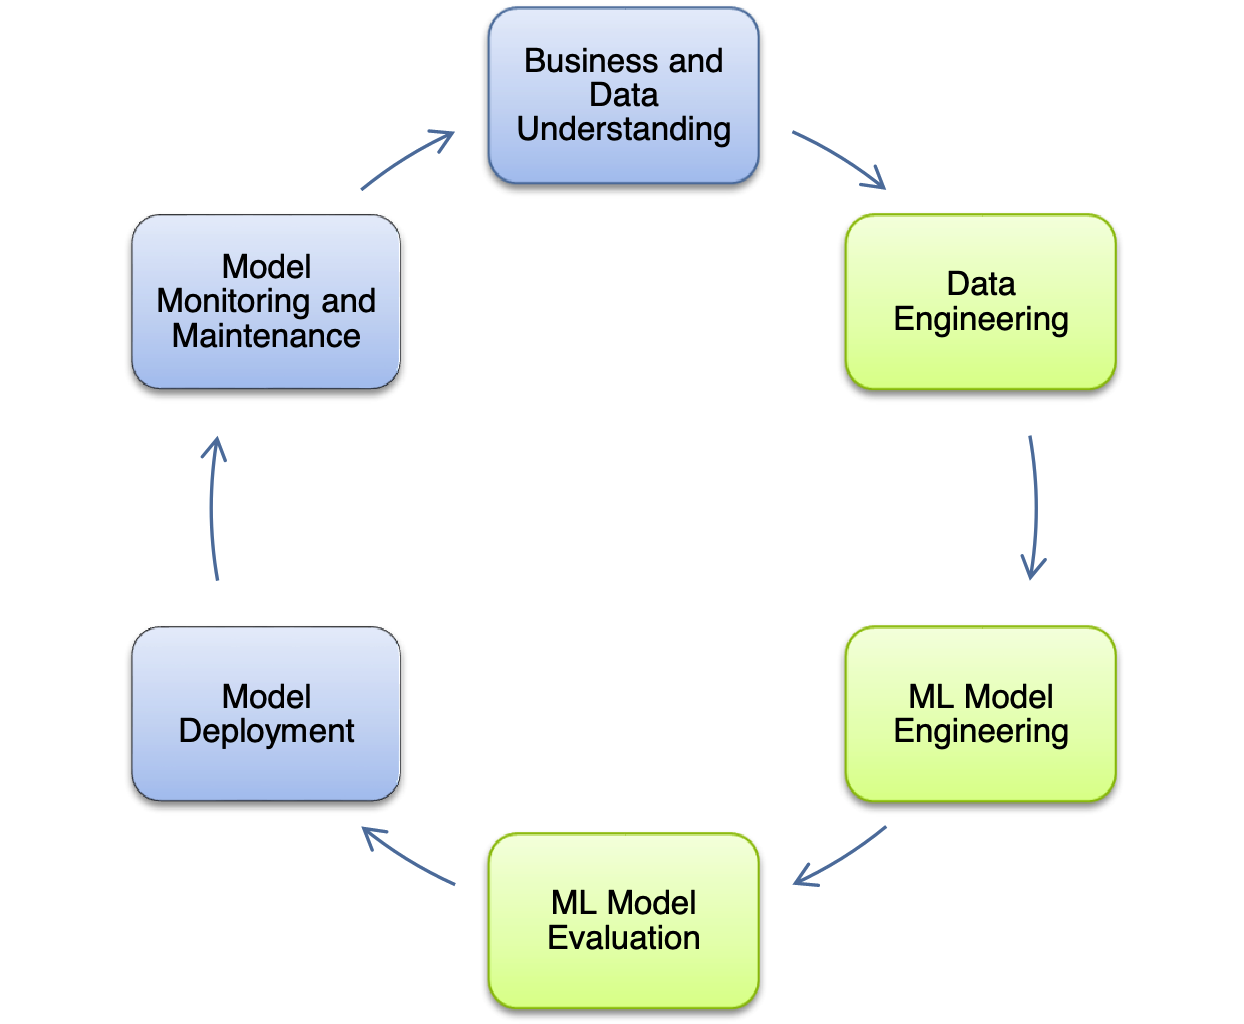
\includegraphics[width=.5\textwidth]{img/crisp.png}
       \caption{The CRISP-ML: Deep Learning Life Cycle as presented in the introductory presentation by Ines Rieger.}
       \label{fig:crisp}
   \end{figure} 

\section{Data Engineering}
During ourur data engineering process we wanted to deal with problems that arise when combining data from multiple sources into a single dataset for model training. Specifically, we identified three key challenges in working with different datasets: combining images from different resolutions and formats, accounting for variations in hand position within each dataset (e.g., hands always positioned in the middle versus positioned elsewhere in the image), and dealing with different contextual backgrounds for the hands (e.g., single-color backgrounds versus real-life image backgrounds). We assumed that reducing the complexity of the datasets was a crucial factor in generating a well-performing model. Thus, our research question was formulated as follows: Does removing the background during the image preprocessing phase benefit the image classification task at hand? This research question will guide our investigation throughout the data engeneering part of the project.


In order to address the data engineering challenges we identified, we combined data from multiple datasets into a single dataset for model training. The training data was created by combining data from several sources, including self-produced images, computer-generated images, and existing datasets from Kaggle. The existing datasets from Kaggle included a dataset of hands with bodies and a dataset of hands from the top. \footnote{\url{https://www.kaggle.com/datasets/drgfreeman/rockpaperscissors}} \footnote{\url{https://www.kaggle.com/datasets/glushko/rock-paper-scissors-dataset}} The computer-generated images were obtained from the TensorFlow datasets catalog. \footnote{\url{https://www.tensorflow.org/datasets/catalog/rock_paper_scissors}} We chose to combine both computer-generated images and real-life images to increase the variety of the training data. Since the testing data was unknown during the data engineering phase of the project, we created a separate validation dataset that was provided by the project, as well as a testing dataset that was also provided by the project. We will refer to these datasets in future discussions as follows: the self-produced images as "custom," the computer-generated images as "cgi," the Kaggle dataset of hands with bodies as "webcam," and the Kaggle dataset of hands from the top as "hands." An overview of the total number of images is presented in Table \ref{tbl:img-origin} and the distributions are shown in Figure \ref{fig:all_data}.


\begin{table}
\caption{Total number of images by source}
\centering
\label{tbl:img-origin}
\begin{tabular}{@{}lllll@{}}
\toprule
\multicolumn{1}{c}{Origin} & Rock & Paper & Scissors & Total \\ \midrule
custom                     & 210  & 205   & 210      & 625   \\
cgi                        & 840  & 840   & 840      & 2520  \\
hands                      & 726  & 712   & 750      & 2188  \\
webcam                     & 752  & 733   & 760      & 2245  \\
Total                      & 2528 & 2490  & 2560     & 7578  \\ \bottomrule
\end{tabular}
\end{table}


\begin{figure}
       \centering
      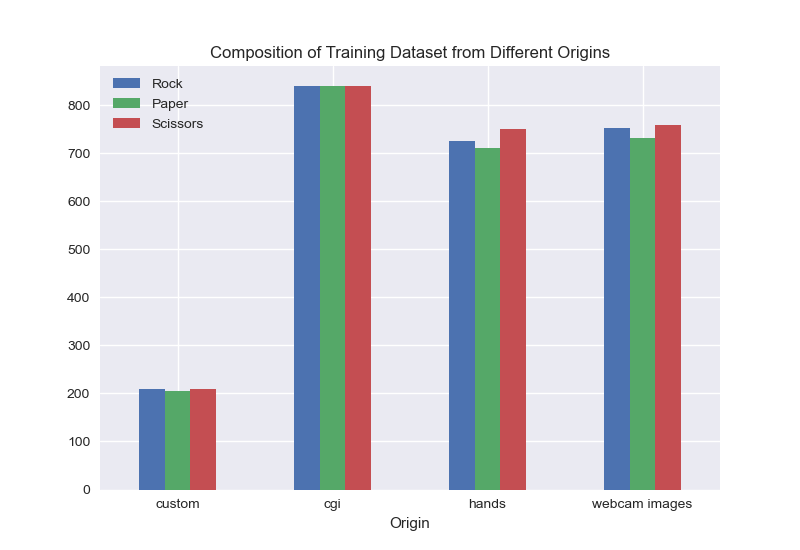
\includegraphics[width=.75\textwidth]{img/ds_analysis/train_ds.png}
       \caption{Individual dataset distribution showing the number of images in each dataset}
       \label{fig:all_data}
   \end{figure} 


To streamline our dataset and remove extraneous background images, we set out to identify Python libraries capable of detecting hands in an image and eliminating the background. After thorough research, we narrowed our focus to three potential options: YOLO-Hand-Detection, rembg, and MediaPipe Hands. Although YOLO-Hand-Detection was able to detect hand positions in real-life images, it was not easily set up and ran the risk of technical difficulties.\footnote{https://github.com/cansik/yolo-hand-detection} Rembg, on the other hand, was readily available and easy to set up, but had shortcomings that resulted in erroneous background removal.\footnote{https://pypi.org/project/rembg/} The purpose of using rembg was to extract the hand from the background and create a uniform image background. Ultimately, we determined that MediaPipe Hands was the most suitable solution, as it can generate a 3D hand model from a 2D image and proved to be highly effective for our purposes.\footnote{https://google.github.io/mediapipe/solutions/hands.html}

MediaPipe Hands is part of MediaPipe, a library developed by Google, which is a versatile tool that provides various functionalities, such as face detection, object recognition, hand detection, and selfie segmentation. We specifically utilized MediaPipe Hands due to its ability to accurately perceive the shape and motion of hands, making it ideal for applications like sign language understanding and hand gesture control. The library is capable of high-fidelity hand and finger tracking, using machine learning to infer 21 3D landmarks of a hand from a single frame \citep{mediapipe}, which allows it to predict a hand skeleton. This is achieved using two models simultaneously: a palm detector that operates on a full input image to locate palms via an oriented hand bounding box, and a hand landmark model that operates on the cropped hand bounding box provided by the palm detector and returns high-fidelity landmarks. Table \ref{tbl:img-hands_percentage} demonstrates the performance of MediaPipe Hands with a hand confidence threshold of 0.1. Based on the results, we determined the performance to be satisfactory for our intended use.

\begin{algorithm}
	\caption{Find the Bounding Box from the MediaPipe Hands Landmarks} 
	\label{alg:bounding-box}
	\begin{algorithmic}[1]
	\State $xHandCords$ $\gets$ $\emptyset$
	\State $yHandCords$ $\gets$ $\emptyset$
		\For {$landmark$ in $handLandmarks$}
			\State $xHandCords$ $\gets$ $xHandCords$ $\cup$ $landmark$.x
			\State $yHandCords$ $\gets$ $yHandCords$ $\cup$ $landmark$.y
		\EndFor
		\State $minX$ = min($xHandCords$)
		\State $minY$ = min($yHandCords$)
		\State $maxX$ = max($xHandCords$)
		\State $maxY$ = max($yHandCords$)
		\State \Return $\{$ $minX$,$minY$,$maxX$,$maxY$ $\}$
	\end{algorithmic} 
\end{algorithm}


For our data engineering problem, we have opted to utilize MediaPipe Hands as the foundation for our preprocessor. This preprocessor is tasked with finding the bounding box around a hand in an image and cropping the image accordingly. Our parameters for image processing include specifying the desired dimensions of the preprocessed image, cropping the image based on the hand position within the image using MediaPipe Hands, removing the background with the rembg library, and converting the images to one-channel greyscale images. The preprocessing steps consist of reading the image using cv2, cropping the image based on the bounding box found with MediaPipe Hands, resizing the image, adding padding if necessary, and converting the image to greyscale using cv2. The method for determining the bounding box to crop the image can be found in Algorithm \ref{alg:bounding-box}. After conducting tests, we selected (300,300) as the desired dimensions which are then scaled down to (64,64) for our final model. Our preprocessor crops images using a hand detection confidence of 0.1, does not remove the background using rembg due to poor performance, and converts the images to greyscale to facilitate one-dimensional model input.


In the final step of our model data engineering, we decided to incorporate data augmentation techniques to improve the generalization of our model. We used simple forms of data augmentation, including random rotations, horizontal and vertical flips, and random affine transformations with shearing and scaling. We implemented these transformations using the standard transformation function provided by PyTorch Data Loader. Our data augmentation function is composed of various transformations, including ToTensor, RandomAffine (shear, scale), RandomRotation, RandomHorizontalFlip, and RandomVerticalFlip. This data augmentation will enable our model to be more robust to variations in the data and increase its performance during testing.

\subsection{Experiment}

Based on the research question, we want to investigate if removing the background (by cropping the images based on the bounding box generated from MediaPipe Hands outcome) during the image preprocessing phase benefits the image classification task. To test this, we will train the same model with and without preprocessed data and then test the performance on a test dataset, both preprocessed and not preprocessed. We hypothesize that the model trained on preprocessed data will perform better than the model trained on non-preprocessed data, as removing the background can reduce noise and improve the model's ability to learn the hand features. Our null hypothesis is that regardless of the preprocessing used, the blackbox model should perform equally on the validation and test dataset in terms of accuracy.



In order to test our research question, we will conduct an experiment where we train a deep learning model on both preprocessed and non-preprocessed data, and then compare their performance on a test dataset. We will use the same preprocessor parameters as before, but will crop images based on MediaPipe Hands with an interval of 0.001 for the validation and training data to obtain the best hand detection. The model parameters will be set with a dropout probability of 0.5, no batch normalization, 100 epochs of training, and a batch size of 64. We will use Adam optimizer with a learning rate of 0.001 and CrossEntropy as the criterion. To compare the models' performances, we will calculate the accuracy of the models on the train, validation, and test data after every 10 epochs of training. We will then compare the differences in accuracy between the two models. The experimental setup is illustrated in Figure \ref{fig:exp-de-setup}.


\begin{figure}
    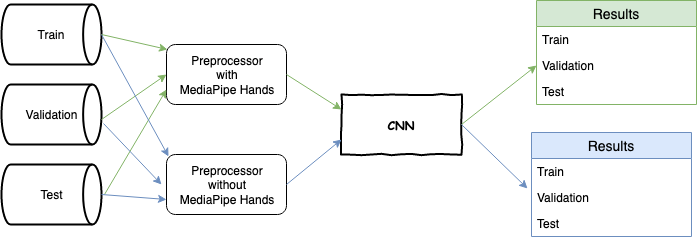
\includegraphics[width=.95\textwidth]{img/experiment/Experiment_Setup.png}
    \caption{Data Engineering experimental setup}
    \label{fig:exp-de-setup}
\end{figure}

\begin{figure}
    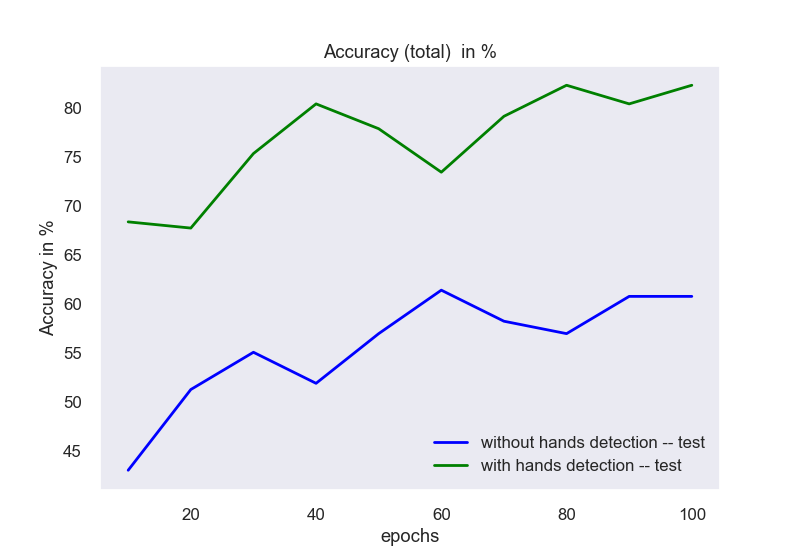
\includegraphics[width=.49\textwidth]{img/experiment/model_comp_10steps__test_acc_total.png}\hfill
    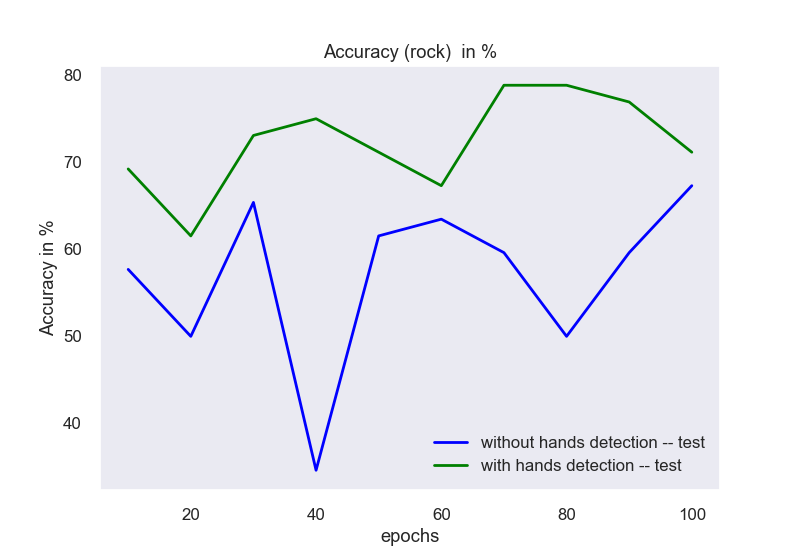
\includegraphics[width=.49\textwidth]{img/experiment/model_comp_10steps__test_acc_rock.png}\hfill
    \\[\smallskipamount]
    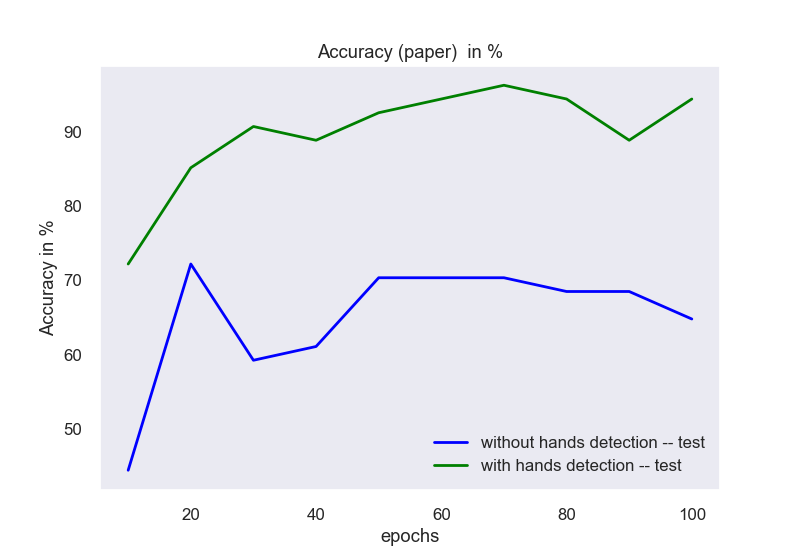
\includegraphics[width=.49\textwidth]{img/experiment/model_comp_10steps__test_acc_paper.png}\hfill
    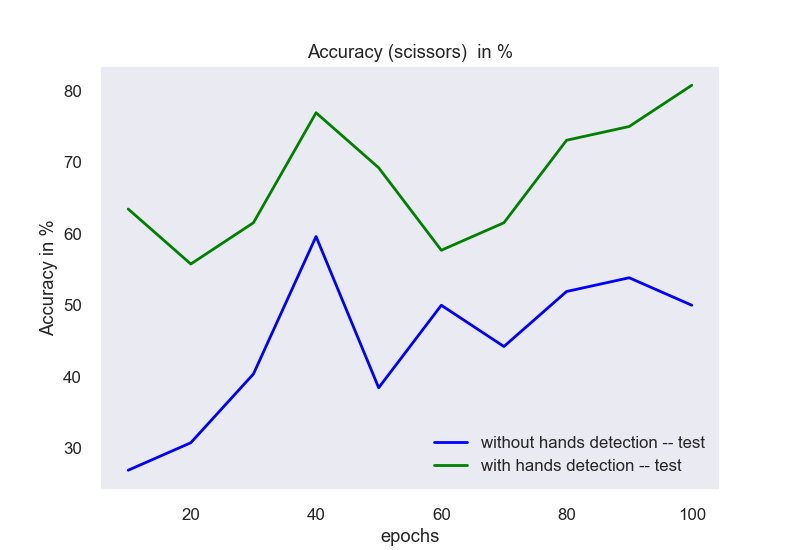
\includegraphics[width=.49\textwidth]{img/experiment/model_comp_10steps__test_acc_scissors.png}\hfill
    \caption{Model performance on test data}
    \label{fig:exp-de-acc-test}
\end{figure}

The results of the experiment are as follows and presented in Figures \ref{fig:exp-de-acc-train}, \ref{fig:exp-de-acc-val} and \ref{fig:exp-de-acc-test}:
\begin{itemize}
	\item Training Data: The model trained on cropped images outperformed the model trained on non-cropped images in terms of accuracy at less training steps. After 60 epochs, the total and category-wise performances of both models were comparable.

    \item Validation Data: The model trained on cropped images consistently outperformed the model trained on non-cropped images in each test model iteration. The total performance of the model trained on cropped images was always better, except for the "rock" category where the model trained on non-cropped images performed slightly better after 100 epochs of training.

    \item Testing Data: The model trained on cropped images consistently outperformed the model trained on non-cropped images in each test model iteration. The model trained on cropped images had much better performance at fewer training steps and remained better over all 100 training epochs. The overall performance of the model trained on cropped images was better.

\end{itemize}
Based on these results, it can be assumed that reducing the complexity of the dataset by removing the background (i.e. unimportant parts of the image) leads to better model performance.

\subsection{Discussion}

The results of our preprocessing pipeline indicate that it was effective in enhancing the quality of the input images for our hand gesture recognition model. However, since we did not apply any statistical tests to our findings, the results only suggest a tendency towards better performance rather than scientifically correct findings.

One issue that arose during the preprocessing stage was the possibility that specific preprocessing techniques could limit the overall performance of the model to the performance of the preprocessing itself. This suggests that more sophisticated preprocessing techniques might be required to improve the performance of the model beyond a certain point. On the other hand, even no preprocessing might be a valid approach but therefore the training data should be increased significantly.

Furthermore, the evaluation of the model on validation and test data revealed that the training data did not sufficiently model the testing and validation data. This might be due to the fact that the training data consisted of CGI and hands with a green background, which is not a common occurrence in real-life scenarios. As a result, it might have been more beneficial to generate much more custom data that better represented the real-life scenarios to improve the performance of the model.

\subsection{Conclusion}

In conclusion, while our preprocessing pipeline was effective in improving the quality of the input images, the results should be interpreted with caution due to the lack of statistical testing. Additionally, the limitation of the preprocessing techniques and the need for more representative training data suggest that another approach should be considered in order to improve the overall performance of the hand gesture recognition model.



\section{Model Engineering} \label{sec:ModelEng}


The performance metric used in the leaderboard was the accuracy on the test set. Thus, one of our main model engineering challenges was to prevent overfitting for the model to be generalizable to unseen images submitted by each team.
The problem of overfitting in machine learning is a common one, especially in deep learning models such as convolutional neural networks. To address this issue, we tried two regularization techniques, namely Dropout and Batch Normalization.
This section aims to investigate the effectiveness of Dropout and Batch Norm in preventing overfitting in our image classification task. 


Our first model was a simple Convolutional Neural Network (CNN). We obtained insufficient results in terms of accuracy, especially on the scissors class. Our hypothesis is that our model was unable to recognize scissors because of the image input size, as we were using 32 x 32 pixels images. Indeed, more pixels are needed to recognize the outline of the fingers making a scissors shape as compared to rock or paper. Therefore, we decided to make input images 64 x 64 pixels instead. We also looked at the literature to improve our model and took inspiration from VGG16 \citep{VGG16}.

\begin{figure}[H]
    \centering
    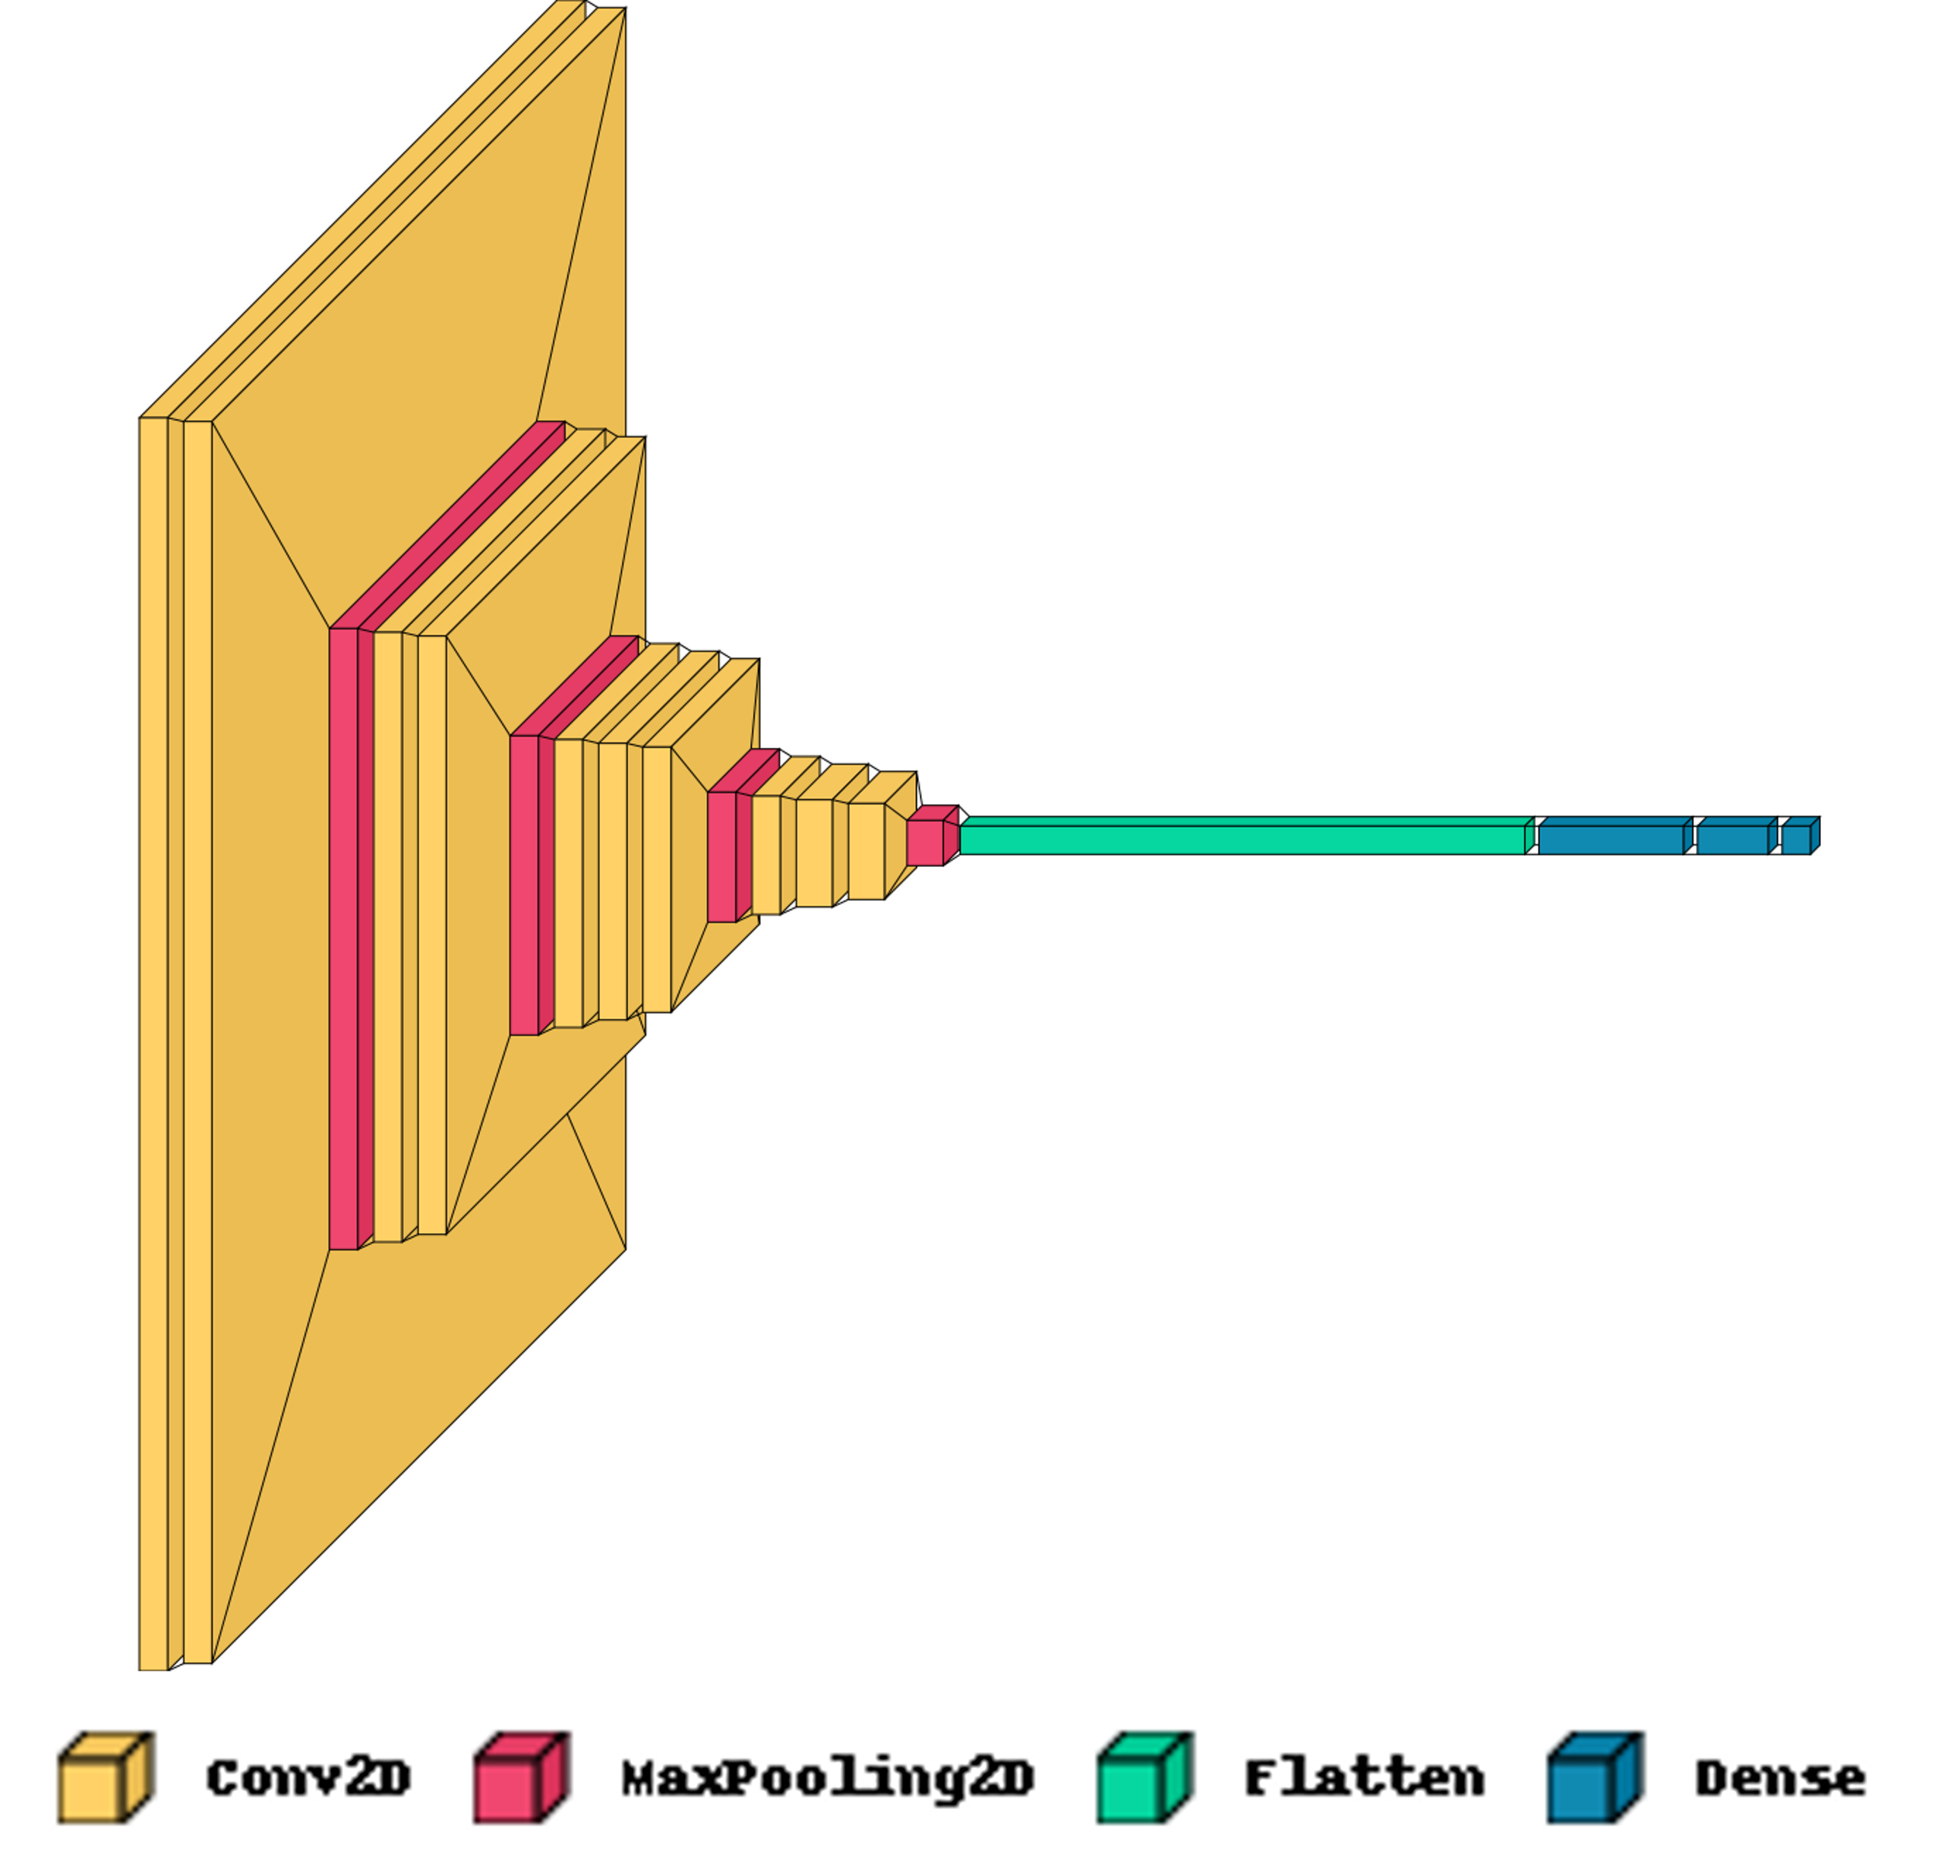
\includegraphics[width=0.5\textwidth]{img/baptiste/model_dropout_false_batchnorm_false.png}
    \caption{Visualization of our model}
\end{figure}


Overfitting is a common problem in machine learning where a model is trained to fit the training data too closely, to the point that it becomes overly specialized and loses its ability to generalize to new, unseen data. This undesirable behavior happens when a model is too complex or has too many parameters relative to the size of the training data. As a result, the model may perform well on the training data, but its performance on the test data is significantly worse. Therefore, overfitting can be diagnosed by splitting the dataset into train, validation and tests sets, and comparing loss and accuracy curves.


Dropout is a regularization technique used in machine learning to prevent overfitting. It works by randomly dropping out a certain percentage of neurons in a neural network during training, which helps to reduce co-adaptation between neurons and makes the network more robust. This means that the network is forced to learn more generalizable features and is less likely to overfit to the training data. Dropout can be applied to any layer in a neural network, including input, hidden, and output layers, and is typically implemented by setting a dropout rate that determines the probability of dropping out each neuron. 


Batch Normalization is a technique used to improve training stability and speed and has also been shown to improve the generalization performance of neural networks. It works by normalizing the input data to each layer of the network so that it has zero mean and unit variance. This helps to alleviate the problem of covariate shift, which occurs when the distribution of input features changes as the network trains. By normalizing the input data, batch normalization helps to ensure that the network can learn more effectively and with fewer training iterations. Batch Norm can be applied to any layer in a neural network, including input, hidden, and output layers, and is typically implemented as a layer in the network architecture.


\subsection{Experiment}

\subsection{Introduction}

The purpose of this experiment is to investigate the impact of Dropout and Batch Norm on overfitting. As explained, overfitting is a common problem in deep learning models, where the model performs well on the training dataset but poorly on the validation and test sets. Dropout and Batch Norm are two popular regularization techniques used to prevent overfitting. Dropout randomly drops out some neurons during training, while Batch Norm normalizes the output of each layer to ensure that the distribution of the input to each layer is consistent. In this experiment, we aim to compare the performance of a neural network trained with and without these regularization techniques.


\subsection{Method}

We trained our neural network for 100 epochs in four different configurations: without any regularization, with Dropout, with Batch Norm, and with both Dropout and Batch Norm. We recorded the classification accuracy and loss on both the training and validation datasets, as well as the accuracy on the test set. The dropout rate was set to 0.5, and the batch size was set to 64. Loss and accuracy curves on training and validation sets recorded during training are available here: Figures \ref{fig:without-regularization}, \ref{fig:with-dropout}, \ref{fig:with-batchnorm}, and \ref{fig:with-dropout-and-batchnorm}.


\subsection{Results}


\begin{figure}[H]
    \centering
    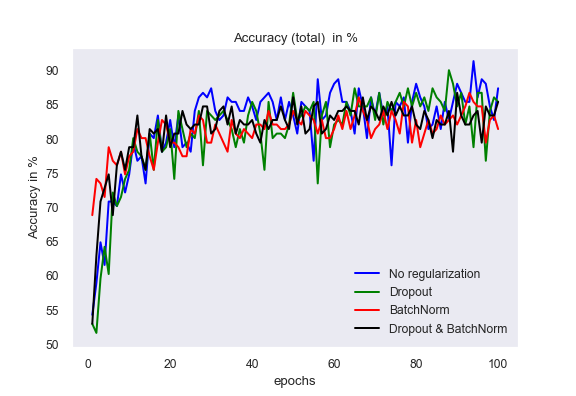
\includegraphics[width=0.9\textwidth]{img/baptiste/baptiste_val_accuracies_comparison.png}
    \caption{Comparison between the four accuracies on validation set}
    \label{val-accuracies}
\end{figure}

Figure \ref{val-accuracies} shows that all accuracies on the validation set are similar, regardless of the regularization technique used. However, Figure \ref{test-accuracies} reveals that the accuracies on the test set are different from each other. The model with Dropout achieves slightly better overall accuracy on the test set than the original model, indicating that Dropout helps to improve the model's generalization ability.



\begin{figure}[H]
    \centering
    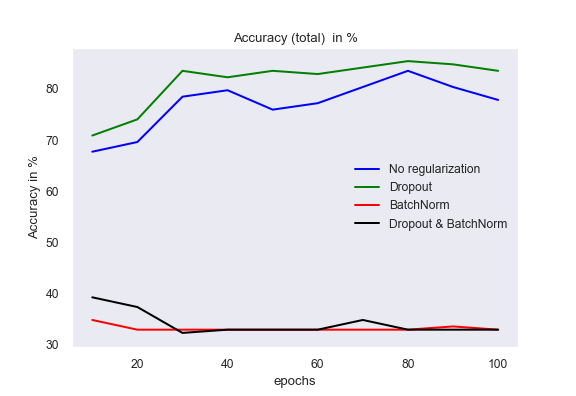
\includegraphics[width=0.9\textwidth]{img/baptiste/baptiste_test_accuracies_comparison.png}
    \caption{Comparison between the four accuracies on test set}
    \label{test-accuracies}
\end{figure}



On the other hand, models incorporating Batch Norm achieve an accuracy level that is notably low, even failing to surpass random chance. This trend shows that Batch Normalization hinders the generalization ability of the model in our case. We came up with several hypotheses to explain this unexpected behavior. During inference, Batch Norm resorts to parameters that were learnt during training based on the statistics of the training data. Therefore, if the discrepancy is substantial between the data distribution of the training set and the test set, then the Batch Normalization layer may not work as well during inference, leading to poor performance. In conclusion, the out-of-domain data contained in the test set explains why Batch Norm worsens model robustness, according to the test accuracy metric.

\subsection{Discussion}

The results of this experiment suggest that Dropout is an effective regularization technique that can help to improve the generalization ability of neural networks. On the other hand, Batch Norm may not always be beneficial, especially when the data distribution of the test set differs substantially from that of the training set.

Note well that the results of this experiment may not generalize to other datasets or models. Further experimentation is necessary to confirm these findings and to explore the effectiveness of other regularization techniques.


\subsection{Conclusion}

In this experiment, we compared the performance of a neural network trained with and without Dropout and Batch Norm. The results show that Dropout helps to improve the generalization ability of the model, while Batch Norm may not always be beneficial. The findings of this experiment can help to inform the choice of regularization techniques in deep learning models. Further research is needed to confirm these results and to explore the effectiveness of other regularization techniques.


\section{Model Evaluation}
\subsection{Basic Model Evaluation} \label{sec:basicEval}
In this section, we will evaluate the previously presented model based on several criteria. For our evaluation, we first look at the performance of the model on the testset that was provided as part of this project. This dataset consists of 158 images, with 54 instances of paper, 52 instances of rock, and 52 instances of scissors.

The evaluation measures indicate that the model performs reasonably well on the classification task, with an overall classification accuracy of 83.54\%. However, the evaluation also reveals some class imbalances, with the precision, recall, and F1-score varying across the three classes. 
For example, the model has a high precision for the rock class (0.911), indicating that when the model predicts the rock class, it is usually correct. However, the recall for the rock class is lower (0.788), indicating that the model misses some instances of the rock class.

Similarly, the model has a high recall for the paper class (0.963), indicating that it correctly identifies most instances of the paper class. However, here the precision for the paper class is lower at 0.754, indicating that the model tends to sometimes predict the paper class incorrectly.
To thoroughly evaluate the performance of the model, we will use precision, recall, F1-score, and accuracy. Precision measures the proportion of true positives among the instances predicted as positive. Recall measures the proportion of true positives among the instances that are actually positive and the F1-score is the harmonic mean of precision and recall. 

To evaluate the accuracy of individual classes we use the One-vs.-rest method, which involves treating the class of interest as the positive class and the remaining classes as the negative class. The model is then evaluated based on its ability to correctly classify instances belonging to the positive class, while ignoring instances belonging to the negative classes. The reported overall classification accuracy of 83.54\%, however, measures the proportion of correctly classified instances among all instances.

To calculate the respective performance metrics, the following equations \citep{metric_formulas} were used:

\begin{equation}
	Precision = \frac{TP}{TP + FP}
\end{equation}

where TP is the number of true positives and FP is the number of false positives.

\begin{equation}
	Recall = \frac{TP}{TP + FN}
\end{equation}

where TP is the number of true positives and FN is the number of false negatives.

\begin{equation}
	F1 = 2 * \frac{Precision * Recall}{Precision + Recall}
\end{equation}

where Precision and Recall are as defined above.

\begin{equation}
	Accuracy = \frac{TP + TN}{TP + TN + FP + FN}
\end{equation}

where TP is the number of true positives, TN is the number of true negatives, FP is the number of false positives, and FN is the number of false negatives.
\newline

We report the evaluation measures for each individual class in Table \ref{tbl:metrics_model}, which includes precision, recall, F1-score, and accuracy.

\begin{table}[h]
	\centering
	\caption{Performance metrics of each individual class}
	\label{tbl:metrics_model}
	\begin{tabular}{@{}lllll@{}}
		\toprule
		Class    & Precision & Recall & F1-Score & Accuracy \\ \midrule
		Rock     & 0.911     & 0.788  & 0.845    & 0.905    \\
		Paper    & 0.757     & 0.981  & 0.855    & 0.886    \\
		Scissors & 0.884     & 0.731  & 0.800    & 0.880    \\ \bottomrule
	\end{tabular}
\end{table}


The overall accuracy of the model is lower than the accuracies for the individual classes, since here only the cases in which the actual and predicted classes match exactly are considered correct. The One-vs.-rest method used for the individual classes does not account for errors that don't involve the current positive class.

To further evaluate, we can look at the confusion matrix of our model's performance on the testset:
\begin{table}[H]
	\centering
	\caption{Confusion matrix of our model on the test data}
	\renewcommand\arraystretch{1.5}
	\setlength\tabcolsep{0pt}
	\begin{tabular}{c >{\bfseries}r @{\hspace{0.4em}}c @{\hspace{0.4em}}c @{\hspace{0.4em}}c @{\hspace{0.4em}}c}
		\multirow{9}{*}{\rotatebox{90}{\parbox{1.4cm}{\bfseries\centering Actual}}} & 
		& \multicolumn{3}{c}{\bfseries Prediction} & \\
		& & \bfseries rock & \bfseries paper & \bfseries scissor & \\
		& \bfseries rock & \MyBox{41} & \MyBox{7} & \MyBox{4} \\
		& \bfseries paper & \MyBox{0} & \MyBox{53} & \MyBox{1} \\
		& \bfseries scissor & \MyBox{4} & \MyBox{10} & \MyBox{38} \\
	\end{tabular}
	\label{tab:CM_model_test}
\end{table}

The confusion matrix (Table \ref{tab:CM_model_test}) shows that the model correctly classified 41 instances of the Rock class, 52 instances of the Paper class, and 38 instances of the Scissors class. The most common error made by the model is to mistake scissors for paper, which occurs in 6.3\% of the cases. This error is understandable because the paper and scissors signs are closely related, and a similar hand gesture can be used to represent both signs. However, this error occurred only in 10 instances, which is a relatively small number of misclassifications. One should note that this result should be interpreted with caution due to the limited size (150 images) of the test set. For a more thorough evaluation a larger and more diverse test set is needed to fully evaluate the model's performance and identify more potential imbalances. \newline
Despite these limitations, the evaluation suggests that the model is reasonably effective at predicting the correct hand sign. In the next section, we describe an experiment that tests the performance of the model on a noisy test set to further evaluate our model and assess its robustness.

\subsection{Experiment - evaluating robustness on distorted images}
\subsubsection{Introduction}
Robustness is a critical aspect of any machine learning model, particularly for image classification tasks. It can be defined as the ability of a model to maintain its performance under naturally-induced image corruptions or alterations \citep{robustness}.

Convolutional neural networks (CNNs) are commonly used for image classification tasks, but they are susceptible to corruption \citep{corruption}. These corruptions can often occur in real-world scenarios due to factors such as a bad internet connection, bad camera quality, or other external factors that cannot be easily controlled. In contrast, humans can easily recognize mildly transformed images caused by noise or blur \citep{corruption}. Therefore, to build a model that can rival human performance, a robust model is required.

A robust model is not only important for achieving high accuracy, but it also ensures the trustworthiness of the model. There is a general scepticism towards artificial intelligence (AI) from the general public \citep{AITrust} and a robustly performing model is an integral part of increasing the trust in AI systems.

To test whether our model is robust and answer our third research question, we conducted an experiment that evaluated the performance of the model on a noisy test set. Specifically, we used two different image modification techniques - Gaussian distortion and random noise - to simulate naturally-induced image corruptions. We compared the performance of our model on our test set with the performance on these noisy datasets. Additionally, we briefly looked into techniques to increase the robustness of our model.

In this experiment, we aimed to determine the impact of image corruptions on the performance of our model and whether it could maintain its performance in real-world scenarios. The results of this experiment will provide valuable insights into the robustness of our model and the potential need for additional optimization to achieve higher performance in real-world settings.

\subsubsection{Method}
To test the robustness of our rock, paper, scissor image classifier model and answer our research question, we used two different image transformations: Gaussian Noise and Random Distortion, which we implemented using the cv2 Python library.

Gaussian Distortion is a common image transformation technique that applies a Gaussian blur to an image. The amount of blur applied is determined by a standard deviation (SD) parameter, which controls the spread of the normal distribution that is used to generate the blur kernel. We applied a SD of 25 on our preprocessed grayscale images, which resulted in a visible but not overly distorted version of the original image.

Random Noise is a different type of transformation that involves randomly removing pixels from an image. To implement this transformation, we assigned each pixel a set chance to be removed. We chose a value of 25\%, which meant that 25\% of the pixels of each image got randomly removed and replaced by a black pixel. 

By using these two transformations on our preprocessed test dataset, we created two additional datasets that included the same images as the original test set, but with the added distortions. This way we can compare the performance of our model on the undistorted dataset with the performance on the two distorted datasets.

To further test whether we could improve the robustness of our model, we also trained the model with noisy data. Specifically, we used the same architecture as described in section \ref{sec:ModelEng} and used the same training set as before but this time it consisted of 70\% non-distorted images and 30\% distorted images with the Random Noise Transformation. This new model allowed us to briefly evaluate the effect of incorporating noisy images to our training data.

Due to issues during the training process and time restraints of the project we stopped the training and used the model produced after only 20 training epochs. This model was the best performing one out of the models trained on noisy data and still provided insight into the effect of using such techniques.

\subsubsection{Results}
Comparing the results presented in section \ref{sec:basicEval} of the model’s performance on the undistorted dataset with the performance on the distorted datasets, we notice a drastic decrease in the performance.

When tested on the dataset with random distortion, the model's accuracy decreased to 0.43. The most noticeable decrease in performance was observed in the scissors class, where the model had difficulty identifying any images as scissors (precision: 0.417, recall: 0.096, F1-score: 0.156). A more detailed overview of the classification distribution can be found in Table \ref{tab:CM_model_randDis}.

When tested on the dataset with Gaussian distortion, the model's total accuracy was 0.49. Here we could observe that the model strongly preferred the paper class and classified most of the images as paper, leading to a recall of 0.907 with a precision of only 0.412. The confusion matrix for this testset can be found in Table \ref{tab:CM_model_GaussDis}.

The evaluation of the model trained on noisy data showed that it performed worse on the undistorted testset (total accuracy: 0.589). However, the model was robust against both distorted datasets, with the same accuracy or higher accuracy than on the undistorted testset.

All the total accuracies are presented in Table \ref{tbl:accuracies_models} below. The exact performance metrics of our standard model on the undistorted testset are shown in Table \ref{tbl:metrics_model} while the remaining metrics on the different datasets can be found in the appendix.

\begin{table}[H]
	\centering
	\caption{Accuracy of our models on different test data}
	\label{tbl:accuracies_models}
	\begin{tabular}{@{}lcc@{}}
		\toprule
		Data                & \multicolumn{1}{l}{Standard Model} & \multicolumn{1}{l}{Model Trained On Noisy Data} \\ \midrule
		Undistorted Testset & 0.835                              & 0.589                                           \\
		Random Distortion   & 0.430                              & 0.652                                           \\
		Gaussian Noise      & 0.494                              & 0.595                                           \\ \bottomrule
	\end{tabular}
\end{table}

\begin{table}[h]
	\centering
	\caption{Confusion matrix of our model on the randomly distorted testset}
	\renewcommand\arraystretch{1.5}
	\setlength\tabcolsep{0pt}
	\begin{tabular}{c >{\bfseries}r @{\hspace{0.4em}}c @{\hspace{0.4em}}c @{\hspace{0.4em}}c @{\hspace{0.4em}}c}
		\multirow{9}{*}{\rotatebox{90}{\parbox{1.4cm}{\bfseries\centering Actual}}} & 
		& \multicolumn{3}{c}{\bfseries Prediction} & \\
		& & \bfseries rock & \bfseries paper & \bfseries scissor & \\
		& \bfseries rock & \MyBox{34} & \MyBox{15} & \MyBox{3} \\
		& \bfseries paper & \MyBox{21} & \MyBox{29} & \MyBox{4} \\
		& \bfseries scissor & \MyBox{23} & \MyBox{24} & \MyBox{5} \\
	\end{tabular}
	\label{tab:CM_model_randDis}
\end{table}

\begin{table}[H]
	\centering
	\caption{Confusion matrix of our model on the testset with Gaussian Noise}
	\renewcommand\arraystretch{1.5}
	\setlength\tabcolsep{0pt}
	\begin{tabular}{c >{\bfseries}r @{\hspace{0.4em}}c @{\hspace{0.4em}}c @{\hspace{0.4em}}c @{\hspace{0.4em}}c}
		\multirow{9}{*}{\rotatebox{90}{\parbox{1.4cm}{\bfseries\centering Actual}}} & 
		& \multicolumn{3}{c}{\bfseries Prediction} & \\
		& & \bfseries rock & \bfseries paper & \bfseries scissor & \\
		& \bfseries rock & \MyBox{18} & \MyBox{31} & \MyBox{3} \\
		& \bfseries paper & \MyBox{5} & \MyBox{49} & \MyBox{0} \\
		& \bfseries scissor & \MyBox{2} & \MyBox{39} & \MyBox{11} \\
	\end{tabular}
	\label{tab:CM_model_GaussDis}
\end{table}


\subsubsection{Discussion}
The results of our experiment showed that the model's performance varied considerably across different datasets, highlighting the importance of robustness to noise and other types of distortion.

We observed that the model trained on undistorted data did not perform well on noisy data, indicating that the model is not robust against noisy data. However, we found that training the model on noisy data improved its robustness to noise. This suggests that training with more diverse data, including noisy data, can help improve the model's robustness.

While the model trained on distorted data was more robust against both types of distortion, we have to note that it did not perform well on any of the test sets. When incorporating noisy data in the training, there are many factors to consider that are beyond the scope of this project. Our attempt at training a model on noisy data was more of a proof of concept, showing that it is possible to increase the model's robustness even though the overall performance was poor. Further investigation is necessary to determine the optimal approach for incorporating noisy data in the training process to achieve both robustness and high performance.

Although we only used two different types of distortion in this study, our results suggest that our model's robustness against one type of distortion can transfer to other types of distortion. Additionally, we acknowledge that our distortion may not be entirely natural, but we attempted to produce noise that is close to naturally occurring noise.


\section{Final Conclusion}

In conclusion, this research project applied the CRISP-ML methodology to the problem of classifying rock, paper, or scissors from images that contain exactly one hand. The project explored the three main steps in the process: Data Engineering, Model Engineering, and Model Evaluation. 
The findings suggest that preprocessing techniques can enhance the quality of input images, although sophisticated techniques might be required to improve performance beyond a certain point. Furthermore, the limitation of the preprocessing techniques and the need for more representative training data suggest that another approach should be considered to improve the overall performance of the hand gesture recognition model. 
The results of the Model Engineering experiment suggest that Dropout is an effective regularization technique that can help improve the generalization ability of neural networks, while Batch Norm may not always be beneficial. 
The Model Evaluation experiment showed that training with more diverse data, including noisy data, can help improve the model's robustness. However, further investigation is necessary to determine the optimal approach for incorporating noisy data in the training process to achieve both robustness and high performance. Overall, this project highlights the importance of applying the CRISP-ML methodology to ensure quality assurance in developing machine learning applications.

\newpage
%\section*{References}


\bibliography{bibliography}
\bibliographystyle{abbrvnat}


%%%%%%%%%%%%%%%%%%%%%%%%%%%%%%%%%%%%%%%%%%%%%%%%%%%%%%%%%%%%%%%%%%%%%%%%%%%%%%%%%%%%%%%%%%%%%%%%%%%%
%% Declaration of Authorship
%%%%%%%%%%%%%%%%%%%%%%%%%%%%%%%%%%%%%%%%%%%%%%%%%%%%%%%%%%%%%%%%%%%%%%%%%%%%%%%%%%%%%%%%%%%%%%%%%%%%

\section*{Declaration of Authorship}
All final papers have to include the following ‘Declaration of Authorship’:

{\parindent 0cm
%%%%%%%%%%%%%%%%%%%%%%%%%%German%%%%%%%%%%%%%%%%%%%%%%%%%%%%%%
\section*{Declaration of Authorship}
Ich erkläre hiermit gemäß § 9 Abs. 12 APO, dass ich die vorstehende Projektarbeit selbstständig verfasst und keine anderen als die angegebenen Quellen und Hilfsmittel benutzt habe. Des Weiteren erkläre ich, dass die digitale Fassung der gedruckten Ausfertigung der Projektarbeit ausnahmslos in Inhalt und Wortlaut entspricht und zur Kenntnis genommen wurde, dass diese digitale Fassung einer durch Software unterstützten, anonymisierten Prüfung auf Plagiate unterzogen werden kann.\\
\vspace{2\baselineskip}
  
Bamberg, \today

\rule[0.5em]{14em}{0.5pt} \hspace{0.25\linewidth}\rule[0.5em]{14em}{0.5pt}
\vspace{1em}
\hspace{4em} (Place, Date) \hspace{0.51\linewidth} (Signature)

Bamberg, \today

\rule[0.5em]{14em}{0.5pt} \hspace{0.25\linewidth}\rule[0.5em]{14em}{0.5pt}
\vspace{1em}
\hspace{4em} (Place, Date) \hspace{0.51\linewidth} (Signature)

Bamberg, \today

\rule[0.5em]{14em}{0.5pt} \hspace{0.25\linewidth}\rule[0.5em]{14em}{0.5pt}
\vspace{1em}
\hspace{4em} (Place, Date) \hspace{0.51\linewidth} (Signature)
}



%%%%%%%%%%%%%%%%%%%%%%%%%%%%%%%%%%%%%%%%%%%%%%%%%%%%%%%%%%%%


%%%%%%%%%%%%%%%%%%%%%%%%%%%%%%%%%%%%%%%%%%%%%%%%%%%%%%%%%%%%


\appendix

\section{Appendix}

\begin{table}[H]
\caption{Percentage of detected hands in images}
\centering
\label{tbl:img-hands_percentage}
\begin{tabular}{@{}lllll@{}}
\toprule
\multicolumn{1}{c}{Origin} & Rock   & Paper  & Scissors & Total  \\ \midrule
custom                     & 95.2\% & 90.7\% & 96.2\%   & 94.1\% \\
cgi                        & 89.0\% & 100\%  & 100\%    & 96.3\% \\
hands                      & 95.9\% & 99.6\% & 94.5\%   & 96.6\% \\
webcam                     & 93,5\% & 96.2\% & 91.8\%   & 93.8\% \\
Total                      & 92.8\% & 98.0\% & 95.6\%   & 95.5\% \\ \bottomrule
\end{tabular}
\end{table}

\begin{figure}[H]
    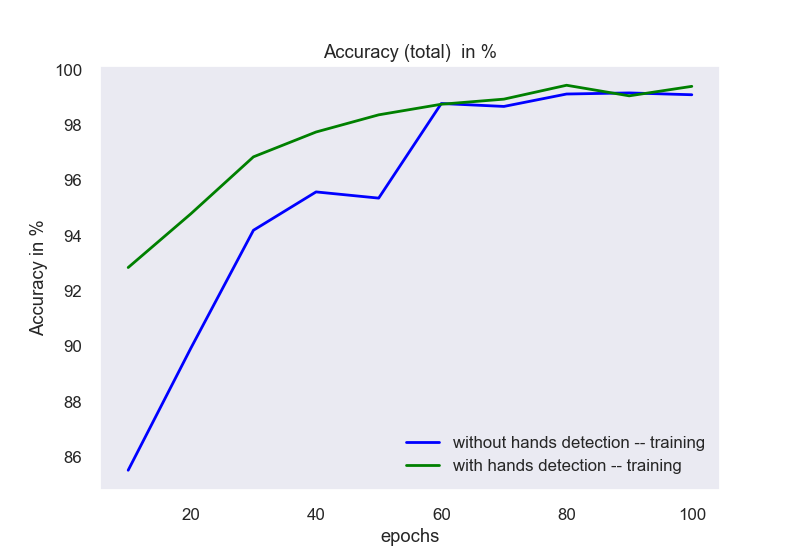
\includegraphics[width=.49\textwidth]{img/experiment/model_comp_10steps__training_acc_total.png}\hfill
    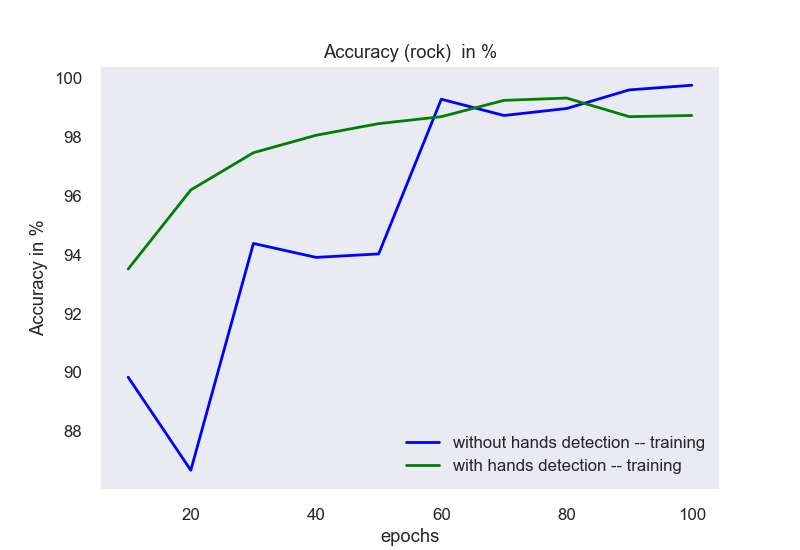
\includegraphics[width=.49\textwidth]{img/experiment/model_comp_10steps__training_acc_rock.png}\hfill
    \\[\smallskipamount]
    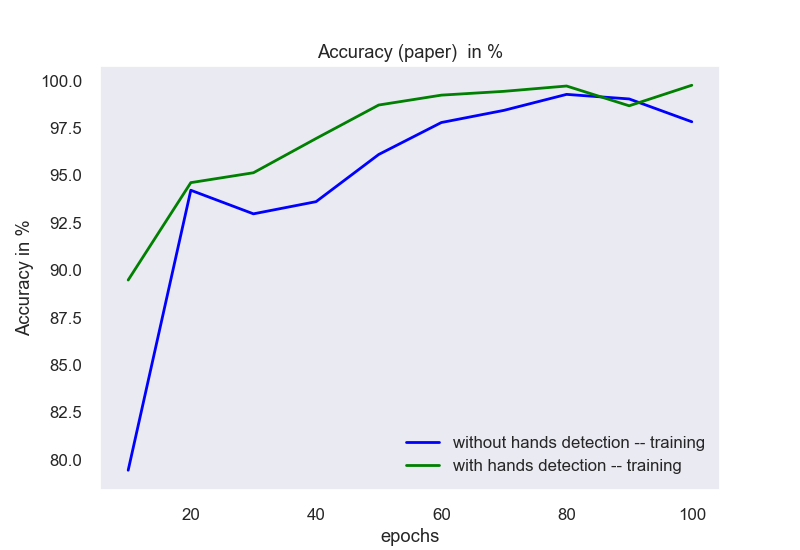
\includegraphics[width=.49\textwidth]{img/experiment/model_comp_10steps__training_acc_paper.png}\hfill
    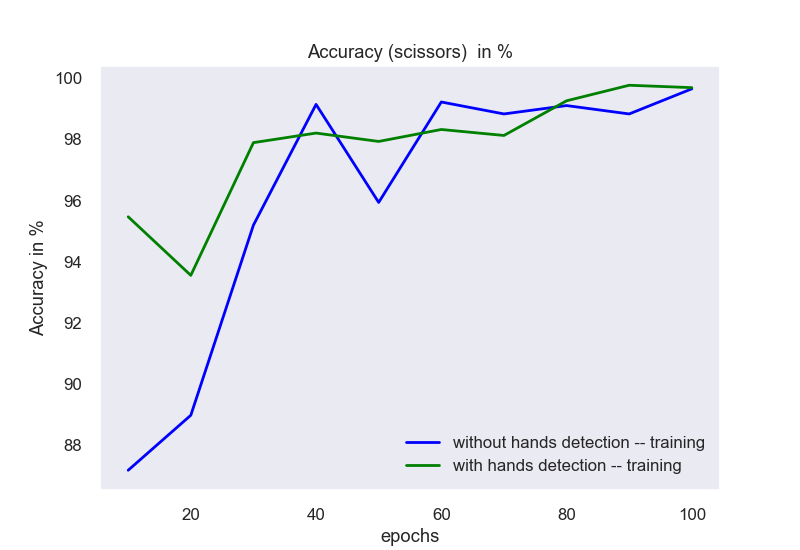
\includegraphics[width=.49\textwidth]{img/experiment/model_comp_10steps__training_acc_scissors.png}\hfill
    \caption{Model performance on training data}
    \label{fig:exp-de-acc-train}
\end{figure}

\begin{figure}[H]
    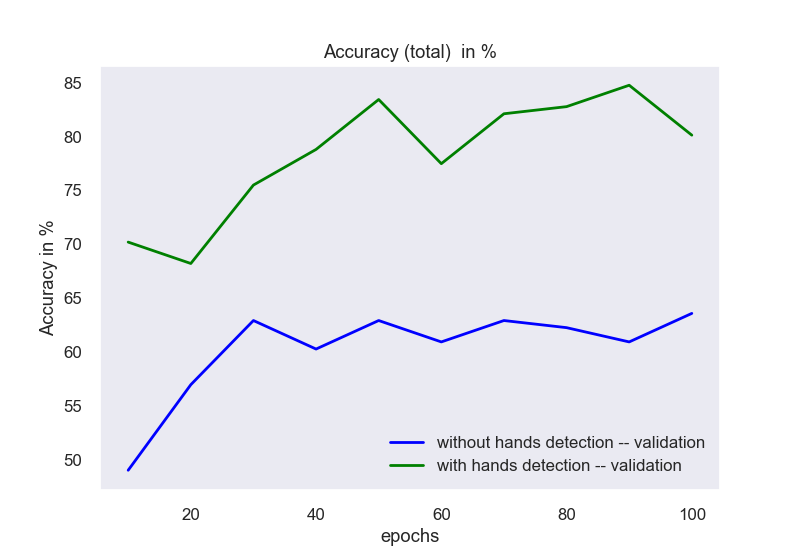
\includegraphics[width=.49\textwidth]{img/experiment/model_comp_10steps__val_acc_total.png}\hfill
    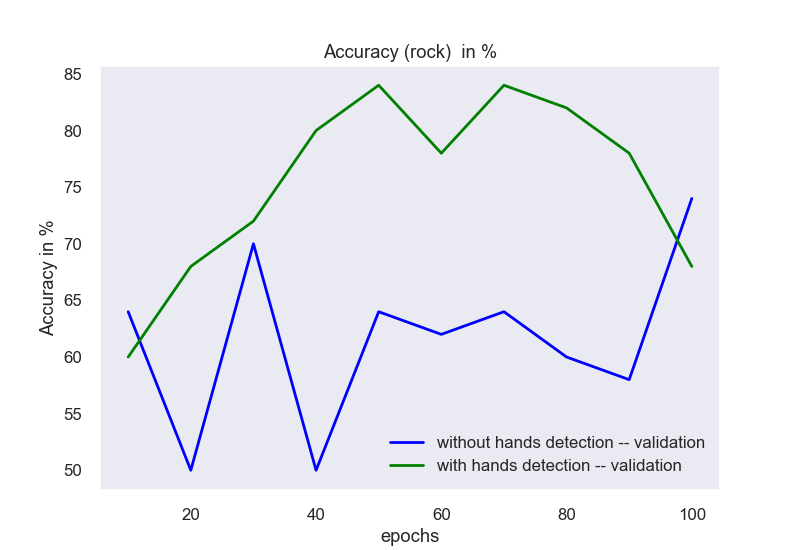
\includegraphics[width=.49\textwidth]{img/experiment/model_comp_10steps__val_acc_rock.png}\hfill
    \\[\smallskipamount]
    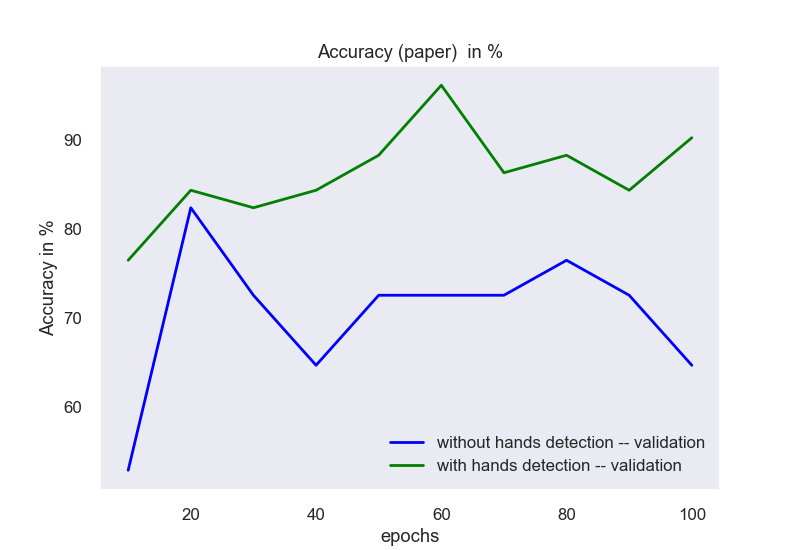
\includegraphics[width=.49\textwidth]{img/experiment/model_comp_10steps__val_acc_paper.png}\hfill
    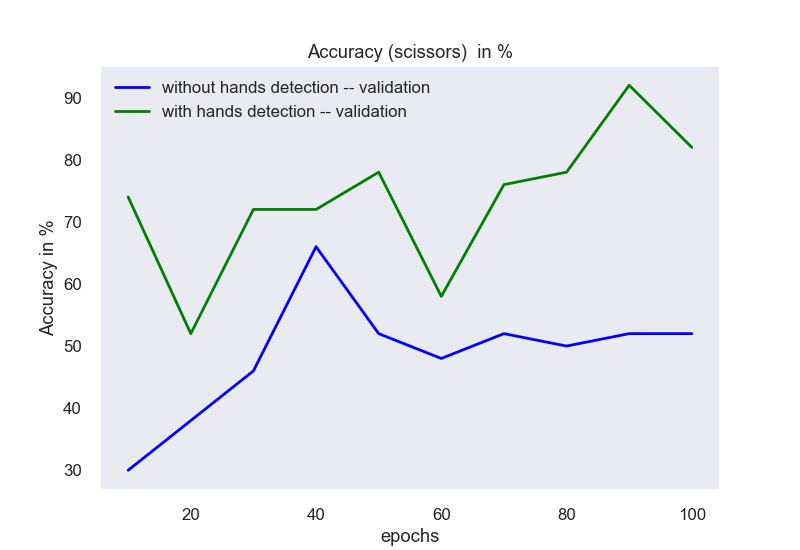
\includegraphics[width=.49\textwidth]{img/experiment/model_comp_10steps__val_acc_scissors.png}\hfill
    \caption{Model performance on validation data}
    \label{fig:exp-de-acc-val}
\end{figure}


\begin{figure}[H]
\centering
\begin{subfigure}{0.5\textwidth}
  \centering
  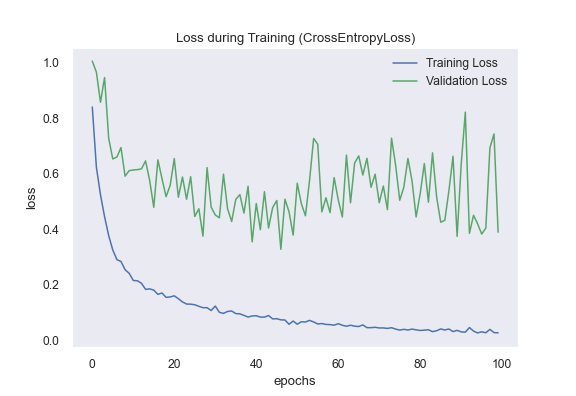
\includegraphics[width=1\linewidth]{img/baptiste/baptiste_100epoches_val_loss__Dropouts_False__BatchNorm_False.png}
  \caption{Training v Validation Loss}
  \label{fig:sub1}
\end{subfigure}%
\begin{subfigure}{0.5\textwidth}
  \centering
  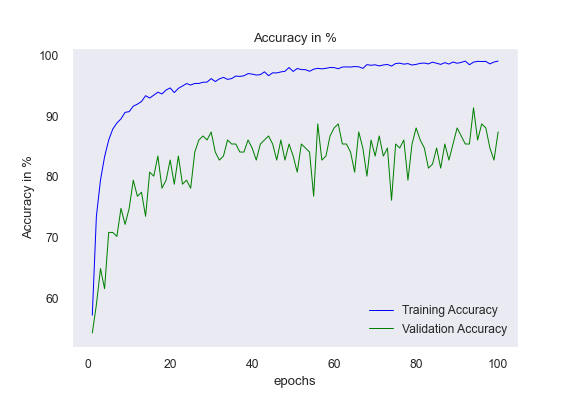
\includegraphics[width=1\linewidth]{img/baptiste/baptiste_100epoches_train_accuracy__Dropouts_False__BatchNorm_False.png}
  \caption{Training v Validation Accuracy}
  \label{fig:sub2}
\end{subfigure}
\caption{Model performance without any regularization}
\label{fig:without-regularization}
\end{figure}

\begin{figure}[H]
\centering
\begin{subfigure}{0.5\textwidth}
  \centering
  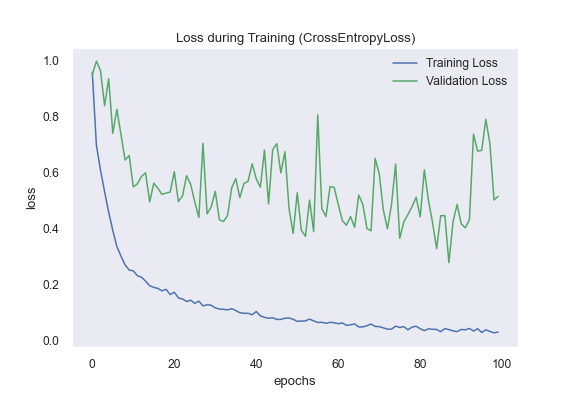
\includegraphics[width=1\linewidth]{img/baptiste/baptiste_100epoches_val_loss__Dropouts_True__BatchNorm_False.png}
  \caption{Training v Validation Loss}
  \label{fig:sub1}
\end{subfigure}%
\begin{subfigure}{0.5\textwidth}
  \centering
  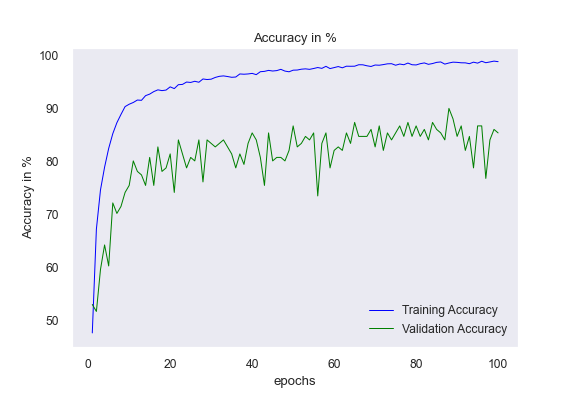
\includegraphics[width=1\linewidth]{img/baptiste/baptiste_100epoches_train_accuracy__Dropouts_True__BatchNorm_False.png}
  \caption{Training v Validation Accuracy}
  \label{fig:sub2}
\end{subfigure}
\caption{Model performance with Dropout}
\label{fig:with-dropout}
\end{figure}

\begin{figure}[H]
\centering
\begin{subfigure}{0.5\textwidth}
  \centering
  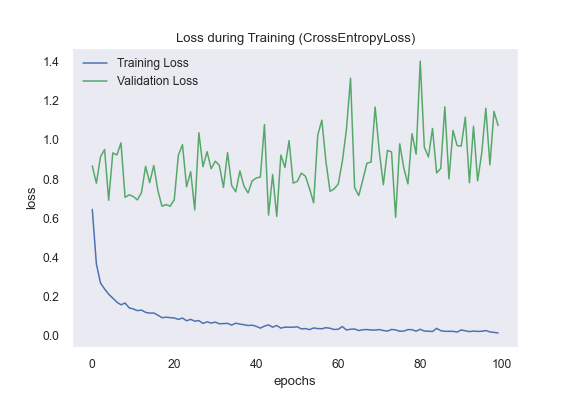
\includegraphics[width=1\linewidth]{img/baptiste/baptiste_100epoches_val_loss__Dropouts_False__BatchNorm_True.png}
  \caption{Training v Validation Loss}
  \label{fig:sub1}
\end{subfigure}%
\begin{subfigure}{0.5\textwidth}
  \centering
  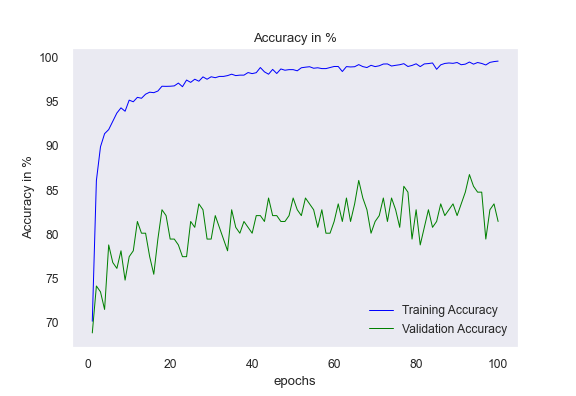
\includegraphics[width=1\linewidth]{img/baptiste/baptiste_100epoches_train_accuracy__Dropouts_False__BatchNorm_True.png}
  \caption{Training v Validation Accuracy}
  \label{fig:sub2}
\end{subfigure}
\caption{Model performance with Batch Norm}
\label{fig:with-batchnorm}
\end{figure}


\begin{figure}[H]
\centering
\begin{subfigure}{0.5\textwidth}
  \centering
  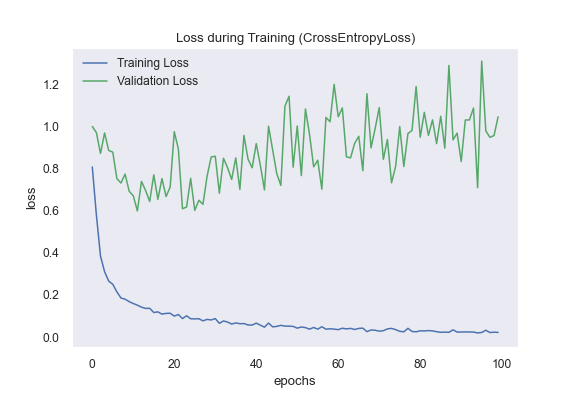
\includegraphics[width=1\linewidth]{img/baptiste/baptiste_100epoches_val_loss__Dropouts_True__BatchNorm_True.png}
  \caption{Training v Validation Loss}
  \label{fig:sub1}
\end{subfigure}%
\begin{subfigure}{0.5\textwidth}
  \centering
  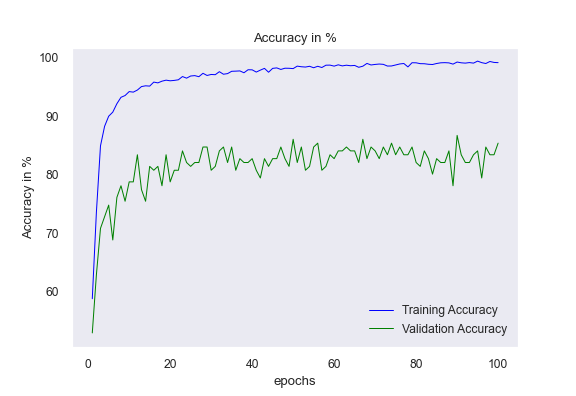
\includegraphics[width=1\linewidth]{img/baptiste/baptiste_100epoches_train_accuracy__Dropouts_True__BatchNorm_True.png}
  \caption{Training v Validation Accuracy}
  \label{fig:sub2}
\end{subfigure}
\caption{Model performance with both Dropout and Batch Norm}
\label{fig:with-dropout-and-batchnorm}
\end{figure}



\begin{table}[H]
	\centering
	\caption{Performance metrics for our standard model on the randomly distorted testset}
	\label{tbl:metrics_model_rm}
	\begin{tabular}{@{}lllll@{}}
		\toprule
		Class    & Precision & Recall & F1-Score & Accuracy \\ \midrule
		Rock     & 0.436     & 0.654  & 0.523    & 0.608    \\
		Paper    & 0.426     & 0.537  & 0.475    & 0.595    \\
		Scissors & 0.417     & 0.096  & 0.156    & 0.658    \\ \bottomrule
	\end{tabular}
\end{table}

\begin{table}[H]
	\centering
	\caption{Performance metrics for our standard model on the testset distorted with Gaussian noise}
	\label{tbl:metrics_model_gauss}
	\begin{tabular}{@{}lllll@{}}
		\toprule
		Class    & Precision & Recall & F1-Score & Accuracy \\ \midrule
		Rock     & 0.720     & 0.346  & 0.468    & 0.741    \\
		Paper    & 0.412     & 0.907  & 0.566    & 0.525    \\
		Scissors & 0.786     & 0.212  & 0.333    & 0.722    \\ \bottomrule
	\end{tabular}
\end{table}

\begin{table}[H]
	\centering
	\caption{Performance metrics for the model trained on 30\% noisy data on the undistorted testset}
	\label{tbl:noisy_model_noDis}
	\begin{tabular}{@{}lllll@{}}
		\toprule
		Class    & Precision & Recall & F1-Score & Accuracy \\ \midrule
		Rock     & 0.542     & 0.865  & 0.667    & 0.715    \\
		Paper    & 0.556     & 0.370  & 0.444    & 0.684    \\
		Scissors & 0.718     & 0.538  & 0.615    & 0.778    \\ \bottomrule
	\end{tabular}
\end{table}

\begin{table}[H]
	\centering
	\caption{Performance metrics for the model trained on 30\% noisy data on the randomly distorted testset}
	\label{tbl:noisy_model_rm}
	\begin{tabular}{@{}lllll@{}}
		\toprule
		Class    & Precision & Recall & F1-Score & Accuracy \\ \midrule
		Rock     & 0.605     & 0.885  & 0.719    & 0.772    \\
		Paper    & 0.641     & 0.463  & 0.538    & 0.728    \\
		Scissors & 0.744     & 0.615  & 0.674    & 0.804    \\ \bottomrule
	\end{tabular}
\end{table}

\begin{table}[H]
	\centering
	\caption{Performance metrics for the model trained on 30\% noisy data on the testset distorted with Gaussian noise}
	\label{tbl:noisy_model_Gauss}
	\begin{tabular}{@{}lllll@{}}
		\toprule
		Class    & Precision & Recall & F1-Score & Accuracy \\ \midrule
		Rock     & 0.592     & 0.808  & 0.683    & 0.753    \\
		Paper    & 0.509     & 0.519  & 0.514    & 0.665    \\
		Scissors & 0.750     & 0.462  & 0.571    & 0.772    \\ \bottomrule
	\end{tabular}
\end{table}

\begin{table}[H]
\caption{Who wrote which part}
\label{tbl:who}
\centering
\begin{tabular}{@{}llll@{}}
\toprule
\multicolumn{1}{c}{Part} & Baptiste   & Benedikt  & Jonas  \\ \midrule
Abstract                     			& & $\surd$  & \\
Introduction                 			&   &  & $\surd$ \\
Data Engineering             			&   &  & $\surd$ \\
Model Engineering 						& $\surd$ & & \\ 
Model Evaluation 						& & $\surd$  & \\
Final Conclusion						& $\surd$ & & \\ 
\bottomrule
\end{tabular}
\end{table}



Here is the link to our GitHub repository : \href{https://github.com/bptstbn/shifumi/tree/ja_final_report}{shifumi}.


\end{document}